% TIPOLOGIA DI DOCUMENTO
\documentclass{report}

% PACCHETTI INSERITI 
\usepackage{graphicx} % Per le immagini
\usepackage{amsmath} % Simboli matematici
\usepackage[hidelinks]{hyperref} % Collegamenti ipertestuali
\usepackage{amssymb} % Simboli matematici 2
\usepackage{tikz}
\usepackage{fancyvrb}
\usepackage{multicol}
\usepackage{geometry}
\usepackage{array}
\usepackage{tabularx} % nel preambolo
\geometry{
 a4paper,
 total={160mm,260mm},
 left=20mm,
 top=18mm,
 }
% RIDENOMINAZIONI
\renewcommand{\chaptername}{Capitolo}
\renewcommand{\contentsname}{Indice}
\renewcommand{\figurename}{Immagine}

% TITOLO, INDICE
\title{\Huge \textbf{{Sistemi Operativi}}}
\author{Damiano Trovato - Lezioni del professore Mario Di Raimondo}
\date{Anno 2024/25, secondo semestre}

\begin{document}
\maketitle
\newpage
\tableofcontents
\newpage

% APPUNTI VERI E PROPRI

\chapter{Il sistema operativo}

\section{Il ruolo del sistema operativo}
Il sistema operativo è un software che ha accesso alle risorse hardware del computer (CPU, RAM, dischi e periferiche), e offre all'utente delle astrazioni semplici per facilitarne la gestione e l'uso. Permette all'utente medio di non dover avere a che fare con i dettagli di basso livello, decisamente più complessi e delicati. \textbf{Rende bello e semplice ciò che dietro le quinte è brutto e complesso}.\\
Tra le astrazioni più note, due casi ben noti sono:
\begin{itemize}
    \item \textbf{Driver dei dispositivi di I/O.}\\
    I driver offrono interfacce semplici per interagire coi dispositivi di input/output. Fornendo delle primitive standard, i driver permettono agli sviluppatori e ai programmi di non dover conoscere troppi dettagli di basso livello relativi ai dispositivi. Sono quindi alla base della compatibilità tra periferiche e calcolatori.
    
    \item \textbf{File.}\\
    L'astrazione più importante dell'intero sistema operativo: mascherano la complessità dei dati situati all'interno di varie porzioni di memoria, sotto forma \textbf{file}. Ciascuno di questi file, ha un'estensione che detta come questo vada interpretato, trattato e gestito.
\end{itemize}

\subsection{Modalità di esecuzione (User-Kernel)}
Il sistema operativo agisce in due modalità:

\begin{itemize}
    \item \textbf{Modalità utente.}\\
    È la modalità con cui vengono eseguiti tutti i software sopra il sistema operativo. Questa modalità offre privilegi limitati al programma, il quale potrà accedere esclusivamente alla memoria ad esso dedicata, e non permette l'accesso a risorse hardware. A tale scopo, tramite delle chiamate di sistema, un programma può chiedere l'intervento dell'sistema operativo, che eseguirà istruzioni in modalità Kernel. Un crash in modalità utente non mette a rischio il resto del sistema.
    \item \textbf{Modalità Kernel.}\\
    O modalità supervisor. I programmi che girano in questa modalità (quali OS, driver e ulteriori software molto specifici), possono accedere alle risorse hardware senza particolari vincoli. È meno restrittiva, ma \textit{da grandi poteri derivano grandi responsabilità}: un crash in modalità Kernel può far fallire l'intero sistema.
\end{itemize}

\newpage

\section{Hardware}
L'hardware è ciò su cui opera il sistema operativo: è quindi fondamentale conoscere la struttura dell'hardware, per studiare i sistemi operativi.

\begin{itemize}
    \item \textbf{CPU}
    \item \textbf{Disk Controller}
    \item \textbf{USB Controller}
    \item \textbf{Graphics Adapter}
    \item Dei \textbf{BUS} che interconnettono le parti precedentemente elencate
\end{itemize}

\subsection{Il processore}
È l'unità di elaborazione centrale (\textit{Central Processing Unit}). Presenta un insieme di registri che possono contenere dei dati. 

\subsubsection{I registri speciali}
Tra questi, alcuni registri particolari sono il PC (\textit{Program counter}), l'SP (\textit{Stack pointer}) e il PSW (\textit{Program Status Word}).
\begin{itemize}
    \item \textbf{Program Counter.}\\
    Il PC contiene l'indirizzo alla prossima istruzione da elaborare.
    \item \textbf{Stack pointer.}\\
    Lo SP contiene delle informazioni necessarie da mantenere per l'esecuzione di un programma (di istruzioni non ancora elaborate).
    \item \textbf{Program Status Word.}\\
    Il PSW contiene informazioni relative a istruzioni di controllo, flag condizionali, modalità di esecuzione della CPU
\end{itemize}
Il sistema operativo deve conoscere bene questi registri, in quanto il parallelismo tra processi ne richiede l'utilizzo. Basti pensare che lo stack pointer tiene un riferimento allo stack delle variabili statiche di ciascun processo e che il program counter fa riferimento alla prossima istruzione da eseguire.

\subsubsection{Il parallelismo}
L'esecuzione parallela di più programmi diventa possibile proprio con l'ausilio di questi registri. Tuttavia, dedicando un quanto di tempo ad ogni processo, c'è un influente (seppur breve) lasso di tempo impiegato per gestire il passaggio dall'esecuzione del processo $n$, a quello $n+1$.

\subsection{Il ciclo di esecuzione dei processi}
\begin{enumerate}
    \item Fetch (nella Fetch Unit)
    \item Decode (nella Decode Unit)
    \item Execute (nella Execute Unit)
\end{enumerate}
I calcolatori moderni permettono di pseudo-parallelizzare l'esecuzione di fasi differenti del ciclo di esecuzione di più processi, avendo parti di hardware dedicate a ciascuna di queste fasi.

\begin{figure}[htp]
    \centering
    \includegraphics[width=0.5\linewidth]{pipelining.png}
    \caption{Esempio di Pipelining}
\end{figure}

In questo modo, ciò che si ottiene è un piccolo (ma importante) guadagno in termini di velocità di esecuzione. Un guadagno di qualche millisecondo diventa molto più importante di fronte a un grande numero di istruzioni.

\subsection{I processori (super)scalari}
Sono costituiti da molteplici unità di fetch, decode ed execute (di cui molte di loro specializzate). Avere molteplici unità, permette di effettuare contemporaneamente la stessa fase di più processi. È richiesta poi la presenza di un holding buffer usata per stabilire l'ordine in cui eseguire le istruzioni. 
\begin{figure}[htp]
    \centering
    \includegraphics[width=0.75\linewidth]{Pipelining e Superscaling a confronto.png}
    \caption{Pipelining e Superscaling a confronto}
\end{figure}

\section{Modalità di esecuzione}
Abbiamo precedentemente individuato due modalità di esecuzione delle\\ istruzioni, ovvero.
\begin{itemize}
    \item \textbf{Modalità utente.}
    \item \textbf{Modalità Kernel.}
\end{itemize}
Nella maggior parte dei sistemi operativi, solo una piccola parte delle istruzioni si effettuano in modalità Kernel. La modalità utente garantisce un uso più sicuro del sistema. Inoltre, ogni chiamata a sistema impiega un determinato lasso di tempo.
\begin{figure}[htp]
    \centering
    \includegraphics[width=0.75\linewidth]{trap.png}
    \caption{Schema generale di chiamata a sistema}
\end{figure}
\\
Il passaggio dalla user mode al Kernel mode è effettuato tramite la \textbf{trap}. Da user mode a Kernel mode è detta \textbf{return}.
\textit{\href{https://www.geeksforgeeks.org/user-mode-and-Kernel-mode-switching/}{Premi qui per una pagina di geeksforgeeks su Kernel mode e User mode.}} 
Tutti gli interrupt sono eseguiti in Kernel mode.

\newpage

\subsection{Più processori}
Avere più processori (o più core) ci permette di distribuire i programmi su più core, facendoli lavorare tutti a pieno regine e ottenendo prestazioni migliori. Tuttavia, il sistema operativo dovrà anche tenere conto di quale processo dovrà essere affidato a quale processore (in funzione dei dati di quel processo già presenti nella cache).
Le caratteristiche dei multiprocessori sono:
\begin{itemize}
    \item \textbf{Alto throughput.}\\
    Massimizza il numero di processi in esecuzione in un determinato lasso di tempo.
    \item \textbf{Economia in scala.}
    \item \textbf{Affidabilità.}
\end{itemize}

\section{Threads}
Un thread è una suddivisione in sottoprocessi dello stesso programma che agiscono in maniera "parallela". Ogni thread potrebbe essere definito come un flusso, ma parte dello stesso processo. Il sistema vede ogni thread come un processore.
\subsection{Multithreading}
Col termine  \textbf{multithreading}, indichiamo la possibilità da parte di un processore di gestire ed eseguire più thread. In ogni istante di tempo è eseguito un solo thread, per questo lo definiremo come uno "pseudo-parallelismo".
\subsection{L'importanza del multithreading}
Il multithreading è alla base dell'esecuzione pseudo-parallela di più processi. I vari thread condividono risorse (dello stesso programma), ma con una gestione ottima (tramite lo scheduler), i processi non competono, ma collaborano, non causando problemi.

\newpage

\section{Memorie}
All'interno di un calcolatore è presente una gerarchia di memorie. Una buona organizzazione delle memorie permette di ottenere un sistema di memorie apparentemente unitario.
\subsection{Gerarchia delle memorie}
Alla cima della piramide troviamo le memorie più veloci, meno capienti e più costose.

\begin{figure}[htp]
    \centering
    \includegraphics[width=0.75\linewidth]{ger2.png}
    \caption{Gerarchia delle memorie}
\end{figure}
\begin{itemize}
    \item \textbf{Registro.}\\
    Contiene un dato su cui si sta effettuando l'operazione corrente.
    \item \textbf{Cache.}\\
    Esistono due tipi di cache. La cache L1 è interna al Core, L2 può essere interna al core, o condivisa tra più core. Contiene dati che sono stati utilizzati recentemente da processi.\\
    La gestione della L2 unica è più difficile, ma è più probabile che un core trovi il dato richiesto da un processo.
    \item \textbf{Memoria Principale.}\\
    Contengono tutte le porzioni di un programma che servono in un determinato istante di tempo, il tempo di accesso in una casella di memoria è diretto (RAM). È volatile, non permanente. Una parte di RAM tuttavia non è volatile, ed è di sola lettura. È la memoria ROM, non è accessibile dall'utente, e contiene tutte le istruzioni relative all'avvio del dispositivo.
    \item \textbf{Disco elettronico.}\\
    Le memorie flash, sono memorie intermedie alla RAM e all'Hard Disk. Sono memorie permanenti e veloci, ma non sono particolarmente capienti. Sono più facilmente soggetti a malfunzionamenti.
    \item \textbf{Disco magnetico e disco ottico.}\\
    Più economico e capiente. È l'hard disk. È costituito da dischi e testine di lettura e scrittura. L'accesso è sequenziale. Ogni disco è suddiviso in tracce e settori.
    \begin{figure}
        \centering
        \includegraphics[width=0.25\linewidth]{disks.png}
        \caption{Struttura di un Hard Disk}
    \end{figure}
    Il tempo di ricerca di un determinato elemento in una posizione casuale del disco magnetico stimata è di 8-10 millisecondi.
    \item \textbf{Memoria virtuale.}\\
    È un meccanismo che, tramite una Memory Management Unit, permette di mappare indirizzi virtuali a indirizzi fisici. La memoria virtuale è presumibilmente più grande della memoria fisica effettiva. Ci permetterà di eseguire tranquillamente programmi parzialmente nella RAM, parzialmente nell'hard disk.
\end{itemize}

\newpage

\section{Strutture di sistemi operativi}
Alcune possibili strutture note per un sistema operativo, sono le seguenti

\begin{itemize}
    \item \textbf{Monolitico.}\\
    Struttura molto comune in cui il sistema operativo, nella sua interezza, è eseguito in modalità Kernel. L'intero sistema è compilato in procedure collegate all'interno di un unico programma. Il fallimento di una singola procedura porta alto rischio di fallimento dell'OS. Il Kernel di Linux è monolitico.

    \item \textbf{A livello (o strati).}\\
    Un'organizzazione gerarchica, in cui ogni livello implementa funzioni impiegando quelle fornite dal livello inferiore.
    Potrebbe avere problemi di performance a causa delle numerose chiamate implicate dal sistema a livelli.\\
    Tuttavia, semplifica la programmazione, in quanto ogni livello si dovrà interfacciare solo con il livello inferiore e superiore. Principio di singola responsabilità.

    \item \textbf{MicroKernel.}\\
    Si minimizzano le operazioni del Kernel, che nel contesto di questi sistemi chiameremo "MicroKernel.". Ottiene maggiore stabilità e minor rischio di fallimento del sistema, delegando il possibile al livello utente. Il microKernel si occuperà quindi di gestire IPC, scheduling dei processi e interrupt di sistema. 
    Questi sistemi operativi suddividono il livello utente in tre sotto-livelli.
    \begin{enumerate}
        \item Programmi utente.
        \item Server.\\
        Si occupa di gestire il file system, gestiscono e distruggono processi. I programmi a livello utente, mandano dei messaggi al livello server, che procederà con una chiamata di sistema POSIX, interfacciandosi ai driver.
        
        \item Driver.\\
        I driver saranno a livello utente: ciò riduce il rischio di fallimenti dell'intero sistema causati da scritture errate in memoria da parte dei driver. Per comunicare con dispositivi I/O, i driver dovranno effettuare delle chiamate di sistema al sistema operativo.
    \end{enumerate}
    
    Queste restrizioni danno responsabilità singole ad ogni singolo componente di questa struttura, seguendo il \textbf{Principle of Least Authority} (POLA).
    
    \item \textbf{Struttura a moduli.}\\
    Simile al Kernel monolitico, ma con la possibilità di caricare moduli in maniera dinamica, che implementano aspetti specifici (file system, driver, etc.).\\
    Il Kernel principale è a funzionalità ridotte, e ogni modulo può invocare altri moduli.\\
    Attenzione: i moduli non comunicano tramite messaggi (come nel sistema microKernel), ma tramite interfacce ben note.

    \item \textbf{Macchine virtuali.}\\
    La virtualizzazione viene gestita dagli \textbf{hypervisor}. Esistono due tipi di Hypervisor:
    \begin{enumerate}
        \item \textbf{Tipo 1.}\\
        Girano direttamente sull'hardware della macchina, ma uno dei sistemi operativi fa da host, monitorando gli altri. Microsoft Hyper-V e VMware sono due esempi.

        \item \textbf{Tipo 2.}\\
        L'OS virtualizzato è un processo di un OS host. VirtualBox è un esempio.
    \end{enumerate}
    I primi hanno dei vantaggi in termini di prestazioni e in termini di sicurezza. Nel tipo 2 aumenta il rischio di \textit{virtual machine escape}.
\end{itemize}


\chapter{Processi}

I computer moderni gestiscono un'alta quantità di processi, che questo sia noto all'utente o meno. Avere più processi, che operano in maniera pseudoparallela e/o parallela (nel caso di più processori) permette di offrire un'esperienza utente migliore nei sistemi operativi interattivi, e performance migliori nei sistemi batch e real-time. 

Il \textbf{modello dei processi} offre un modello concettuale semplice per descrivere e gestire il problema del parallelismo.


\section{Modello dei processi}

\underline{Definiamo un \textbf{processo} come un'\textbf{istanza} di \textbf{esecuzione} di un programma.}
Un processo in memoria, \\presenta i seguenti elementi:

\begin{itemize}
    \item Sezione di \textbf{testo contenente il codice} eseguibile.
    \item Sezione \textbf{dati}, contenenti \textbf{variabili globali e statiche}.
    \item \textbf{Heap} e \textbf{Stack}, rispettivamente per la memoria allocata dinamicamente, e per quella relative alle chiamate a funzione.
\end{itemize} 

\begin{figure}[htp]
    \centering
    \includegraphics[width=0.25\linewidth]{process.png}
\end{figure}

Inoltre, ad ogni processo è associato un \textbf{Process Control Block}, ovvero un record all'interno di una \textbf{Tabella dei Processi} gestita dal Sistema Operativo, di cui parleremo dopo.

\subsection{Disambiguiamo processi e programmi}
Un programma, è del codice presente in memoria. Un processo, è un'istanza in esecuzione di un programma. Due istanze dello stesso programma sono due processi distinti.

\subsection{CPU virtuale, pseudoparallelismo}
Il modello a processi semplifica il ragionamento pensando nel seguente modo: ad ogni processo è garantita una personale \textbf{CPU} (chiaramente virtuale) e uno spazio di \textbf{memoria} (virtualmente) \textbf{personale} e (virtualmente) \textbf{infinito}. Ogni \textbf{processo} è (virtualmente) \textbf{sequenziale}.

Nel pratico, la CPU dedica un \textbf{quanto} di tempo al processo $n$, poi al processo $n+1$, poi al processo $n+\dots$, secondo delle regole e dei termini che scopriremo durante il corso.\\
Ad ogni cambio di processo a cui la CPU si dedica, avviene un \textbf{cambio di contesto}: le istruzioni da eseguire dalla CPU e le risorse da usare vengono cambiate, in funzione dell'istanza del programma da eseguire, (concettualmente) passando da una CPU virtuale alla prossima.\\
Otteniamo quindi uno \textbf{pseudo-parallelismo}.
In un sistema single-core lo pseudo-parallelismo è fondamentale per gestire un sistema complesso di multiprogrammazione. Ricordiamo che, anche quando apparentemente stiamo eseguendo un solo programma, i processi in background sono molteplici, e di fondamentale importanza.


\section{Creazione processi}
In questa sezione diamo un'occhiata alle circostanze che portano alla creazione di un nuovo processo, e al come questo avvenga (in termini di chiamate di sistema) nei vari sistemi operativi.

\subsection{Quando viene creato un processo?}
La \textbf{creazione} di un processo può avvenire in quattro principali circostanze.
\begin{itemize}
    \item All'avvio del sistema, col \textbf{boot}.\\
    Solitamente il processo iniziale ha Process Id-1. È la radice dell'albero dei processi. Gli ulteriori processi di avvio saranno inizializzati dal processo radice, o da altri processi, tutti appartenenti allo stesso albero.

    \item Da parte di un \textbf{processo padre}, tramite chiamate di sistema.\\
    Nel caso dei multiprocessori, da dei vantaggi: delegare responsabilità differenti a più processi, permette di distribuire il carico di lavoro su più CPU, soffrendo anche di meno da chiamate bloccanti e circostanze simili.
    
    \item Per un'azione dell'\textbf{utente}.\\
    All'interno dei sistemi interattivi.

    \item Inizio di un job in sistemi batch.\\
    Avviene quando lo scheduler del sistema batch, secondo la propria politica di scheduling e le risorse disponibili del sistema, seleziona un job dalla coda di job da eseguire. 
\end{itemize}

\subsection{Daemon}
In sistemi che supportano la multiprogrammazione, esistono processi detti \textbf{processi daemon}. Sono processi eseguiti in background che gestiscono attività di vario tipo, garantendo servizi all'utente. Non sono associati a utenti in particolari, ma hanno funzioni specifiche. Prendendo come esempio due processi, mail-client e mail-server:
\begin{itemize}
    \item \textbf{Mail client.}\\
    Offre un'interfaccia rivolta all'utente.
    \item \textbf{Mail server.}\\
    Resta in ascolto su un socket, risvegliandosi all'arrivo di una e-mail, garantendo un servizio al processo client.
\end{itemize}

La maggior parte dei processi all'avvio sono processi daemon in background.

\newpage

\subsection{Creare processi nei vari sistemi operativi}

Dipendentemente dal sistema operativo, le metodologie di creazione e di terminazione dei processi, variano.
\begin{itemize}
    \item \textbf{Sistemi UNIX.}\\
    \verb|fork| del processo padre, con successiva chiamata \verb|execve| (o una chiamata analoga). La chiamata di sistema \verb|fork|, da parte di un processo, crea una copia identica di quest'ultimo, con lo stesso spazio degli indirizzi, permessi e file aperti. Questo processo può usare la chiamata chiamata a sistema \verb|execve| per cambiare la propria immagine di memoria ed eseguire un nuovo programma, diventando un processo diverso da quello da cui è stato forkato.
    
    Il sistema UNIX può risalire al processo padre.
    \item \textbf{Alla Windows.}\\
    È richiesta una singola chiamata di sistema, \verb|Win32(CreateProcess)| con 10 parametri.
    \begin{itemize}
        \item Nome del programma da eseguire.
        \item Parametri della riga di comando da passargli.
        \item Vari attributi di sicurezza.
        \item Bit di controllo relativo a file aperti ereditati.
        \item Informazioni di priorità.
        \item Specifiche di creazione della finestra (del programma, se presente).
        \item Un puntatore alla struttura in cui viene restituita al chiamante l'informazione riguardo al processo appena creato.
    \end{itemize}
    È un'istruzione atomica che fornisce già un nuovo processo con una propria immagine di memoria.
\end{itemize}

\subsection{Esempio nei sistemi UNIX}
Supponiamo di avere una shell, da cui avviamo il programma \verb|sort|.\\
Dietro le quinte, la shell creerà un nuovo processo, copia di se stessa, con gli stessi permessi e spazio degli indirizzi, tramite la syscall \verb|fork|. Verrà poi chiamata la syscall \verb|execve| (o simile) per modificare l'immagine di memoria di questo nuovo processo (figlio dello shell), utilizzando il programma \verb|sort| come "blueprint" di se stesso. Avendo comunque accesso allo stesso spazio di memoria del padre e agli stessi permessi, ha la possibilità di accedere agli stessi file del padre e di reindirizzare il suo output a quest'ultimo (banalmente, lo standard output!).

\newpage

\section{Terminazione di un processo}

La terminazione di un processo, può avvenire in varie circostanze.

\begin{itemize}
    \item \textbf{Uscita normale (condizione volontaria).}\\
    È la terminazione normale di un programma. I processi terminano per scelta dell'utente o da parte di un altro processo tramite una chiamata di sistema:
\begin{itemize}
    \item \textbf{UNIX.}\\
    \verb|exit|
    \item \textbf{Windows.}\\
    \verb|ExitProcess|
\end{itemize}

Ritorna un exit status.

\item \textbf{Uscita su errore (volontario).}\\
È una terminazione concepita dal programma.

\item \textbf{Errore critico (involontario).}\\
È un meccanismo automatico che scatta quando il processo cerca di eseguire azioni anomale o illegali, come violazioni relativi allo spazio di indirizzamento (tentativo di scrittura in zone read-only), divisioni per zero, etc..\\ In quel caso, l'hardware fa scattare un'eccezione, causando un'interruzione del processo.\\
In questo caso, non avviene un tentativo di recoveri.

\item \textbf{Terminato da un altro processo (involontario)}
Avviene quando un processo \textbf{richiede} la terminazione di un altro processo.
\begin{itemize}
    \item \textbf{UNIX.}\\
    \verb|kill|
    \item \textbf{Windows.}\\
    \verb|TerminateProcess|
\end{itemize}
Solitamente avviene quando i due processi avvengono nello stesso utente \\(l'amministratore può tuttavia uccidere i processi di qualsiasi utente).

\end{itemize}

\subsection{Soft Kill, Hard Kill}
Le richieste di terminazioni possono essere di due tipi:
\begin{itemize}
    \item \textbf{Soft Kill.}\\
    Viene mandato un segnale specifico al programma di cui vogliamo effettuare la chiusura. Il programma può rispondere con una routine può o addirittura rifiutare la chiusura.
    \item \textbf{Hard Kill.}\\
    Consiste nella terminazione del processo a priori.
\end{itemize}

\newpage

\section{Ciclo di vita di un processo}
I possibili stati di un processo possono essere astratti tramite un automa a stati finiti, cui stati sono i seguenti:
\begin{itemize}
    \item 3 stati principali, \verb|ready, running, blocked|
    \item I 2 stati iniziali e finali \verb|new, terminated|
\end{itemize}

\begin{figure}[htp]
    \centering
    \includegraphics[width=1\linewidth]{fsm.pdf}
    \caption{Un diagramma a stati che descrive il ciclo di vita di un processo}
\end{figure}


\subsection{Gli stati di un processo}
Nello studio degli stati dei processi, supporremo sempre di avere una sola CPU.

\subsubsection{New e Terminated}
Sono due stati meno importanti.\\
Lo stato \verb|new| fa riferimento alla fase di predisposizione delle risorse in funzione dell'apertura del processo.\\
Lo stato \verb|terminated| fa riferimento alla fine dell'esecuzione di un processo.

\subsubsection{Ready}
\textbf{Il processo è pronto ad usare la CPU}. Il sistema operativo si occupa della gestione dei processi nello stato \verb|ready|, che sono contenuti in una coda chiamata \textbf{coda dei processi}, di cui parleremo dopo.\\
La coda dei processi viene usata dallo scheduler per stabilire che processo far passare allo stato \verb|running|. All'interno della coda si trovano i riferimenti ai processi.
Effettuata la scelta, il sistema ha il compito di mettere in esecuzione il processo.
\newpage

\subsubsection{Running}
Con i presupposti dell'unica CPU, \textbf{solo un processo può essere nello stato di running}. Dallo stato di \verb|running|, in funzione di scenari diversi, si passerà a stati differenti.

\begin{itemize}
    \item \textbf{Attesa di evento o Input/Output (Blocked).}\\
    Il processo \textbf{ha bisogno di una chiamata a sistema} (e quindi di una \textbf{trap}), in quanto necessita l'\textbf{aiuto del sistema operativo}.\\
    Alcune chiamate di sistema sono dette "\textbf{lente}". Sono chiamate che solitamente, hanno tempi di gestione più lenti delle istruzioni della CPU.
    \\
    \textit{\href{https://unix.stackexchange.com/questions/14293/difference-between-slow-system-calls-and-fast-system-calls}{Clicca qui per leggere sulle chiamate lente e veloci}}.\\
    Se la CPU è assegnata ad un processo su cui è stata effettuata una \textbf{syscall lenta}, il processo transita nello stato \verb|blocked| (tirandolo fuori dalla coda dei processi). Rienterà nella coda e tornerà allo stato \verb|ready| quando arriverà la risposta alla sua syscall lenta.
    Nota bene! Questo non vuol dire che il processo verrà ri-eseguito istantaneamente: bensì, tornerà nello stato \verb|running| a discrezione dello scheduler. 
    \item \textbf{Interrupt (Ready).}\\
    Fa passare dallo stato di \verb|running| allo stato di \verb|ready|.\\ È contemplato nei sistemi che presentano il meccanismo di \textbf{prelazione}. In questo scenario, un ipotetico processo $A$ in stato \verb|ready| può ottenere la CPU, attualmente utilizzata da un processo $B$ in stato \verb|running|, aspettando un determinato interrupt mandato da un clock di sistema. Questo farà tornare $B$ allo stato \verb|ready|, per non fargli "monopolizzare" la CPU.
\end{itemize}

\subsection{Prelazione}
È l'operazione tramite cui un processo viene temporaneamente interrotto e portato al di fuori della CPU, senza alcuna cooperazione da parte del processo stesso, al fine di permettere l'esecuzione di un altro processo.
\underline{Nei sistemi interattivi è fondamentale la prelazione}, nessun processo deve poter monopolizzare la CPU. 
Ad esempio: un processo occupa la CPU per un quanto\footnote{unità di misura che useremo per indicare il tempo dedicato ad un determinato processo} di tempo. Se il processo non entra nello stato blocked entro la fine del quanto di tempo, passa nello stato di ready, e la CPU viene dedicata ad un altro processo.

Questo evento è gestito tramite un \textbf{interrupt} legato ad un clock di sistema (e viene quindi mandato dall'hardware): ad ogni segnale di clock, viene invocata una routine della CPU, che verifica se il processo ha superato il quanto di tempo dedicato. In tal caso, il processo entra nello stato di ready.


\subsection{Busy wait vs Blocking wait}
Notiamo che il meccanismo dello stato di blocking evita lo spreco di cicli di CPU. La CPU non controlla ad ogni step se la condizione di attesa è stata soddisfatta, ma è il processo cui risposta viene attesa, che segnala di poter far tornare il processo bloccato nello stato \verb|ready|.

\
\newpage


\section{Tabella dei processi}
È una struttura dati dinamica, usata dal sistema operativo per gestire i processi, e che contiene al suo interno dei record, chiamati Processo Control Block (PCB). Quando un nuovo processo viene creato, viene allocato un PCB. Quando un processo termina, viene deallocato.

\subsection{PCB - Process Control Block}
Sono i record della tabella dei processi. Ne è presente uno per ogni istanza di un programma, e quindi uno per processo. Contengono al loro interno:

\begin{itemize}
    \item \textbf{Stato} del processo.
    \item \textbf{Process ID} (PID).
    \item \textbf{Program Counter} (PC).
    \item Contenuto dei \textbf{registri della CPU}, salvato per ripristinarne il contenuto nel momento \\dell'esecuzione.
    \item Limiti di memoria (\textbf{spazio degli indirizzi}).
    \item \textbf{File aperti}.
    \item \textbf{Processi imparentati}.
\end{itemize}

In generale, le PCB contengono tutto ciò che possa servire allo \textbf{scheduler} per effettuare i \textbf{cambi di contesto}, noti anche come \textbf{Context Switch}, che approfondiremo più avanti.
\begin{figure}[htp]
    \centering
    \includegraphics[width=1\linewidth]{pcbetc.png}
\end{figure}

\subsection{Scheduler}
È il componente del Kernel che sceglie quale processo deve essere eseguito, dalla coda dei processi pronti. La scelta del processo da eseguire in un determinato istante non è banale, e stabilire le proprietà variano spesso dal sistema (personal computer, sistemi real-time, batch e HPC avranno priorità differenti).

\newpage

\section{Coda e accodamento}
I processi nello stato \verb|ready| sono pronti ad usare la CPU, e sono situati in una coda, chiamata \textbf{ready queue}. Quando un processo viene selezionato dallo scheduler, a questo è assegnata la CPU, in un processo chiamato \textbf{process dispatching}.

\subsection{La coda dei processi pronti}
La tabella dei processi è una struttura dinamica al cui interno sono situati i PCB. La coda dei processi pronti è (chiaramente) un sottoinsieme della tabella dei processi, che coinvolge tutti i processi nello stato \verb|ready|. Sarebbe ridondante proporre una struttura a parte per la coda, considerando che esiste già la tabella dei processi (che in quanto dinamica, è implementata come una lista doppiamente concatenata).

Ne consegue che il modo migliore per gestire la cosa, è sfruttare direattamente la tabella dei processi, aggiungendo dei puntatori dedicati invece alla coda dei processi pronti.

\subsection{Diagramma di accodamento}
Sono tre le circostanze in cui, un processo nello stato \verb|running| può incorrere.

\begin{figure}[htp]
    \centering
    \includegraphics[width=1\linewidth]{queueueueu.png}
    \caption{Casi di riaccodamento di un processo in esecuzione}
\end{figure}

\begin{itemize}
    \item \textbf{Richiesta di I/O}: il processo verrà inserito in una coda I/O di attesa.
    \item \textbf{Una fork di un processo} genereerà un processo figlio, di cui il padre attenderà la terminazione.
    \item Il processo viene rimosso dallo stato di running a causa di un \textbf{interrupt}, \textbf{tornando così nella coda dei processi pronti} (quindi, nello stato \verb|ready|).
\end{itemize}
Il sistema operativo gestisce delle code per ciascuna di queste circostanze.

\subsubsection{Prelazione}
L'ultimo caso, include anche il \textbf{timer interrupt}: il clock di sistema, alla conclusione di un timer, invia un segnale di interrupt (detto \textbf{clock interrupt}), in modo da non far monopolizzare la CPU ad alcun processo. Questo meccanismo è presente nei sistemi operativi che supportano la \textbf{prelazione}. La prelazione è fondamentale in sistemi utente multiprogrammati.

\chapter{Thread}

\section{Introduzione al modello a thread}
Detto anche modello a thread multipli, permette di gestire l'esecuzione di un singolo processo su \textbf{più flussi di esecuzione indipendenti}. Il disegno sottostante rappresenta il nostro modello:

\begin{center}
\tikzset{every picture/.style={line width=0.75pt}} %set default line width to 0.75pt        

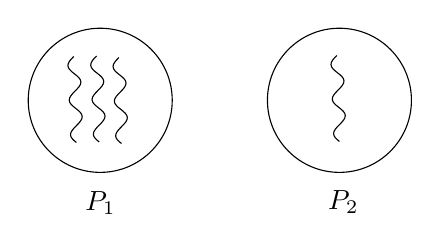
\begin{tikzpicture}[x=0.75pt,y=0.75pt,yscale=-1,xscale=1]
%uncomment if require: \path (0,300); %set diagram left start at 0, and has height of 300

%Shape: Ellipse [id:dp07477881872708148] 
\draw   (36.07,44.78) .. controls (36.07,25.6) and (51.6,10.05) .. (70.76,10.05) .. controls (89.92,10.05) and (105.45,25.6) .. (105.45,44.78) .. controls (105.45,63.96) and (89.92,79.5) .. (70.76,79.5) .. controls (51.6,79.5) and (36.07,63.96) .. (36.07,44.78) -- cycle ;
%Shape: Ellipse [id:dp6981516240796339] 
\draw   (151.32,44.78) .. controls (151.32,25.6) and (166.85,10.05) .. (186.01,10.05) .. controls (205.17,10.05) and (220.7,25.6) .. (220.7,44.78) .. controls (220.7,63.96) and (205.17,79.5) .. (186.01,79.5) .. controls (166.85,79.5) and (151.32,63.96) .. (151.32,44.78) -- cycle ;
%Shape: Wave [id:dp06184582088810897] 
\draw   (58,23.67) .. controls (56.53,25.15) and (55.13,26.57) .. (55.18,28.08) .. controls (55.24,29.59) and (56.74,30.77) .. (58.32,32) .. controls (59.9,33.23) and (61.4,34.41) .. (61.45,35.92) .. controls (61.51,37.43) and (60.11,38.85) .. (58.63,40.33) .. controls (57.16,41.82) and (55.75,43.24) .. (55.81,44.75) .. controls (55.87,46.26) and (57.37,47.44) .. (58.95,48.67) .. controls (60.52,49.9) and (62.03,51.08) .. (62.08,52.59) .. controls (62.14,54.1) and (60.74,55.52) .. (59.26,57) .. controls (57.79,58.49) and (56.38,59.91) .. (56.44,61.42) .. controls (56.49,62.82) and (57.8,63.94) .. (59.25,65.08) ;
%Shape: Wave [id:dp8460485311920296] 
\draw   (69,23.42) .. controls (67.53,24.9) and (66.13,26.32) .. (66.18,27.83) .. controls (66.24,29.34) and (67.74,30.52) .. (69.32,31.75) .. controls (70.9,32.98) and (72.4,34.16) .. (72.45,35.67) .. controls (72.51,37.18) and (71.11,38.6) .. (69.63,40.08) .. controls (68.16,41.57) and (66.75,42.99) .. (66.81,44.5) .. controls (66.87,46.01) and (68.37,47.19) .. (69.95,48.42) .. controls (71.52,49.65) and (73.03,50.83) .. (73.08,52.34) .. controls (73.14,53.85) and (71.74,55.27) .. (70.26,56.75) .. controls (68.79,58.24) and (67.38,59.66) .. (67.44,61.17) .. controls (67.49,62.57) and (68.8,63.69) .. (70.25,64.83) ;
%Shape: Wave [id:dp11269480405206944] 
\draw   (79.75,24.17) .. controls (78.28,25.65) and (76.88,27.07) .. (76.93,28.58) .. controls (76.99,30.09) and (78.49,31.27) .. (80.07,32.5) .. controls (81.65,33.73) and (83.15,34.91) .. (83.2,36.42) .. controls (83.26,37.93) and (81.86,39.35) .. (80.38,40.83) .. controls (78.91,42.32) and (77.5,43.74) .. (77.56,45.25) .. controls (77.62,46.76) and (79.12,47.94) .. (80.7,49.17) .. controls (82.27,50.4) and (83.78,51.58) .. (83.83,53.09) .. controls (83.89,54.6) and (82.49,56.02) .. (81.01,57.5) .. controls (79.54,58.99) and (78.13,60.41) .. (78.19,61.92) .. controls (78.24,63.32) and (79.55,64.44) .. (81,65.58) ;
%Shape: Wave [id:dp6518132342393432] 
\draw   (184.75,23.17) .. controls (183.28,24.65) and (181.88,26.07) .. (181.93,27.58) .. controls (181.99,29.09) and (183.49,30.27) .. (185.07,31.5) .. controls (186.65,32.73) and (188.15,33.91) .. (188.2,35.42) .. controls (188.26,36.93) and (186.86,38.35) .. (185.38,39.83) .. controls (183.91,41.32) and (182.5,42.74) .. (182.56,44.25) .. controls (182.62,45.76) and (184.12,46.94) .. (185.7,48.17) .. controls (187.27,49.4) and (188.78,50.58) .. (188.83,52.09) .. controls (188.89,53.6) and (187.49,55.02) .. (186.01,56.5) .. controls (184.54,57.99) and (183.13,59.41) .. (183.19,60.92) .. controls (183.24,62.32) and (184.55,63.44) .. (186,64.58) ;

% Text Node
\draw (62.37,87.6) node [anchor=north west][inner sep=0.75pt]  [xscale=1,yscale=1] [align=left] {$\displaystyle P_{1}$};
% Text Node
\draw (179.35,87.02) node [anchor=north west][inner sep=0.75pt]  [xscale=1,yscale=1] [align=left] {$\displaystyle P_{2}$};
\end{tikzpicture}
\end{center} %% IMMAGINE THREAD E PROCESSI

dove $P_1,P_2$ sono processi, e le linee all'interno sono i thread. \textbf{Processi diversi non hanno risorse comuni}, sono indipendenti. I \textbf{thread dello stesso processo hanno invece risorse condivise}. Possono offrire servizi paralleli allo stesso processo, permettendo di ottenere performance migliori e/o meno circostanze bloccanti per l'intero processo. Il motivo per cui preferiamo scomporre i processi in thread e non in processi, è relativo allo spazio degli indirizzi condiviso: il context switch tra thread dello stesso processo è più veloce del context switch di due processi separati

\subsubsection{Non possiamo lavorare a singoli thread? \textit{What if - Esempi vari}}
Immaginiamo di avere la possibilità di gestire \textbf{un solo thread per processo}: 

\begin{itemize}
  \item Un text editor: il rendering del file si bloccherebbe ad ogni salvataggio. Il controllo lessicale bloccherebbe la scrittura. 
  \item Un web server: le richieste possono essere gestite solo una ad una. Una richiesta molto onerosa blocca tutte le altre richieste, creando una coda non indifferente, e riducendo il throughput.
\end{itemize}

Avere la possibilità di gestire più flussi di esecuzione, è fondamentale per avere programmi più complessi e responsivi.


\section{I thread}
Un thread è un flusso di esecuzione indipendente di un processo. I thread dello stesso processo hanno lo stesso PID (Process ID).
Ciascun thread è caratterizzato da:
\begin{itemize}
    \item \textbf{Program Counter}
    \item \textbf{Registri}
    \item \textbf{Stack}
    \item \textbf{Stato}: \verb|blocked|, \verb|ready| o \verb|running|.
\end{itemize}

E condividono tutto il resto, ossia spazio di indirizzamento, heap, memoria globale, codice\footnote{che nel libro è indicato con "testo"} e file aperti.

\subsection{Piccolo prezzo da pagare: gestione dei thread}
I thread sono flussi indipendenti, ma non isolati nativamente o protetti vicendevolmente. Ciò consegue che due o più thread che operano sulle stesse risorse, potrebbero causare anomalie di fronte a determinate circostanze, di cui parleremo più avanti. Le chiameremo \textbf{race condition}, o \textbf{corse critiche}.

\subsection{Scheduling dei thread}
Lo scheduler si occuperà della scelta del thread del programma che andrà ad occupare la CPU in un determinato istante. Nei sistemi moderni, lo scheduler tratta i thread come processi a se stanti.

\subsubsection{Context switch sui thread}
Il concetto di \textbf{context switch}\footnote{Ricordiamo cos'è il context switch: consiste nel salvataggio del contesto corrente e nel ripristino del contesto entrante.} avviene anche nell'ambito dei thread. Quando avviene il context switch, l'MMU viene riprogrammata sul thread entrante.\\
Il context switch dei thread avviene sempre tra thread dello stesso processo: rispetto al context switch tra processi, quello tra thread è molto più veloce, in quanto i thread condividono lo stesso spazio di memoria, sollevando l'MMU dal dover riprogrammare lo spazio di indirizzamento.

\subsection{Cambiamenti di stato dei thread}
I cambiamenti di stato dei thread sono analoghi a quelli dei processi. Possono essere nello stato di \verb|running|, \verb|ready| o \verb|blocked|.

\begin{figure}[htp]
    \centering
    \includegraphics[width=0.50\linewidth]{threadstates.png}
\end{figure}

\subsection{Operazioni tipiche sui thread}
\begin{itemize}
    \item \verb|thread_create|.\\
    Un thread ne crea un altro.
    \item \verb|thread_exit|.\\
    Il thread chiamante termina.
    \item \verb|thread_join|.\\
    Un thread si sincronizza con la fine di un altro thread.
    \item \verb|thread_yield|.\\
    Il thread chiamante rilascia volontariamente la CPU.
\end{itemize}

\newpage

\section{Introduzione al multicore programming}
I thread permettono di ottenere performance migliori sui sistemi multithread e multicore.
Se in un sistema single-core possiamo ottenere un esecuzione \textit{interleaved} e pseudo parallela, su un sistema multi-core possiamo ottenere un parallelismo vero e proprio: in entrambi i casi si parla di concorrenza, ma solo in uno dei due, il parallelismo è vero e proprio (anche se, le intuizioni relative allo pseudo-parallelismo rimangono sempre fondamentali, in quanto il numero di thread eseguibili in parallelo è limitato).

\subsection{Programmazione multicore}
Progettare programmi che sfruttino le architetture multicore non è banale.

\begin{itemize}
    \item \textbf{Separazione dei task.}
    \item \textbf{Bilanciamento.}\\
    Ottenere una suddivisione dei task ben bilanciati, significa gestire bene le responsabilità e le durate temporali dei task dei thread, che dovranno essere bilanciate in maniera opportuna.
    \item \textbf{Suddivisione e dipendenze dei dati.}\\
    Bisogna analizzare i dati di cui i thread avranno bisogno, individuare le risorse dati condivise e se esistono dipendenze tra i dati.\\
    Cosa intendiamo con dipendenza? Il thread $A$ ha bisogno di un dato elaborato dal thread $B$.
    \item \textbf{Test e debugging.}\\
    La fase più odiata probabilmente. È molto complesso ottenere un programma multithread corretto: altrettando difficile è riuscire a stanare, in fase di testing, tutti i casi limite e le circostanze problematiche che possiamo riscontrare nell'esecuzione del codice.
\end{itemize}


\subsection{Sistemi single-core vs multi-core}
I thread permettono di suddividere l'esecuzione di un programma in più flussi. In sistemi single-core, si ottiene un'esecuzione alternata. In sistemi multicore, si ottiene un'esecuzione parallela (ma anche alternata) vera e propria.

\begin{figure}[htp]
    \centering
    \includegraphics[width=0.8\linewidth]{multithread.drawio (1).pdf}
\end{figure}


\subsection{Tipologie di thread}

\begin{itemize}
    \item \textbf{Thread a livello utente.}\\
    1-a-molti, artificialmente creati a livello utente su un unico flusso di esecuzione suddiviso da uno scheduler. Non devono essere supportanti nativamente dal Kernel.
    \item \textbf{Thread a livello Kernel.}\\
    1-a-1, con un thread a livello utente associato ad ogni thread a livello Kernel. devono essere supportanti nativamente dalla CPU.
    \item \textbf{Thread in modalità ibrida.}\\
    È un modello ibrido, detto molti-a-molti.
\end{itemize}

\newpage

\section{Thread a livello utente}
Detto anche \textbf{modello 1-a-molti}, è utile per lavorare su un Kernel che non ha supporto nativo ai thread. Il sistema operativo non sa cos'è un thread: dato un programma, offre la possibilità di operare su un solo flusso di esecuzione. Tuttavia, tramite opportune librerie, è possibile introdurre dei thread a livello utente, a pari del nostro codice. Sarà poi l'implementazione dei thread da parte della libreria, a gestire l'esecuzione concorrente. 

\subsection{Come fa la CPU a saltare tra thread?}
La chiave per lo switch tra thread è una primitiva che abbiamo introdotto precedentemente:\\ \verb|thread_yield|. Essa effettuerà il salvataggio dei registri sulla tabella dei thread, anche essa nello spazio utente.

\subsection{Criticità sui thread a livello utente}
Il modello 1-a-molti è molto versatile, ma presenta delle criticità.

\paragraph{Chiamate bloccanti}
Le chiamate lente, o bloccanti, bloccano tutti i thread del processo. Questo, avviene a carico del sistema operativo, che nell'effettivo non conosce i thread a livello utente. \textbf{Per il sistema operativo, i thread a livello utente non sono altro che codice di un unico processo.} Ciò è molto grave, soprattutto rispetto a operazioni lente sul disco o operazioni di I/O.

Una soluzione?  La chiama a sistema \verb|select|, che verifica se una chiamata, in un determinato istante e contesto, sarà bloccante, ossia a condizione della chiamata lenta soddisfatta.

\begin{itemize}
    \item Se la chiamata \textit{sarà} bloccante, l'esecuzione procederà regolarmente.
    \item Se la chiamata \textit{non sarà} bloccante, si usa la primitiva \verb|thread_yield| su quel thread. Ciò avverrà fino a quando quella chiamata non sarà più bloccante.
\end{itemize}

Esempio semplice: $t_1$ aspetta un input da tastiera. La richiesta input è una syscall lenta se non è già presente testo nel buffer d'input. \verb|thread_yield| su $t_1$ per farne rilasciare la CPU. Questo passaggio si ripete fino a quando non sarà presente testo nel buffer. In tal caso, la \verb|select| darà il via libera per il \underline{non} richiamo della \verb|thread_yield| su $t_1$. Implementiamo così un meccanismo a livello utente per far rilasciare la CPU ad un thread.
Anche i \textbf{page-fault} causano l'interruzione di un processo: a malincuore, anche in questo caso non è possibile fermare esclusivamente il thread.

\paragraph{Possibilità di non rilascio}
Un thread potrebbe non rilasciare la CPU. Un thread non può forzare un altro thread a rilasciare la CPU. La libreria che implementa i thread dovrà gestire in maniera opportuna questo aspetto.

\subsection{I punti di forza}
\paragraph{Scheduling personalizzato}
I thread a livello utente non possono sfruttare la prelazione, in quanto quest'ultima sfrutta degli interrupt di sistema. Per quanto questa potrebbe risultare come una limitazione, la natura a livello utente di questi thread, permette di implementare un meccanismo di priorità personalizzata dei processi contestuale e meno asettica di quella a sistema operativo: più versatilità.

\paragraph{Dispatching senza trap}
L'operare interamente a modalità utente di questi thread, evita i tempi di attesa relativi alle chiamate a sistema, notoriamente lunghe. I thread a livello utente sono notoriamente più veloci e meno costosi.

\newpage

\section{Thread a livello Kernel}
Detto anche "modello 1-a-1". Sfrutta le possibilità del sistema operativo. La thread table diventa a livello Kernel, ed unica per tutti i processi, in quanto è proprio il Kernel a supportare i thread. Nel pratico sono addirittura unificate, in quanto i processi saranno definiti come sottoinsiemi di elementi della tabella dei thread.

\begin{figure}[htp]
    \centering
    \includegraphics[width=0.75\linewidth]{multithread.drawio.pdf}
\end{figure}

\subsection{Vantaggi di questo modello}
In questo modello, una chiamata bloccante può bloccare un solo e unico thread, eliminando la più grande criticità dei Kernel a livello utente!

\subsection{Svantaggi}

\paragraph{Il context switch}
In questo caso, il context switch è più lento, come conseguenza dell'utilizzo di \verb|trap|.

Il context switch più lento è quello tra thread di due processi differenti.
Più veloce sarà quello tra due thread imparentati, in quanto non richiederà la riprogrammazione dell'MMU.

\paragraph{Operazioni costose}
Creare e distruggere thread diventa un'operazione molto più costosa. Creare thread Kernel frequentemente può rallentare esponenzialmente il sistema. 


\section{Modello ibrido}
Detto anche "molti-a-molti". Prende il meglio dal mondo dei thread-utente e dei thread-Kernel.

\subsection{Come si procede nel modello ibrido?}
Si prevede un dato numero di thread Kernel, fisso e non troppo grande. Successivamente, si assegna ad ogni thread Kernel uno o più thread utente.
Un esempio? Due thread Kernel, tre thread utente. I due thread utente sullo stesso thread Kernel vanno sul controllo ortografico e sul salvataggio (sono operazioni dietro le quinte), l'ultimo thread utente assegnato ad un singolo thread Kernel si occupa della GUI (più delicata e responsiva all'utente).

\section{I thread nei nostri sistemi operativi}
Quasi tutti gli OS supportano i thread a livello Kernel, ma usano primitive diverse. I thread utente sono supportati tramite apposite librerie.

\subsection{pthreads}
La libreria \verb|pthreads|, basata sullo standard POSIX, introduce thread a livello utente e funzioni per renderne la gestione quanto più semplice possibile,  econ un'interfaccia univoca. Univoca in quanto il codice sarà compilabile e funzionante su molteplici sistemi operativi: ciò che succede dietro le quinte cambia, ma il codice sorgente e i risultati rimangono analoghi.

\newpage

\chapter{Interprocess Communication}

Gestire in maniera opportuna la comunicazione tra $n$ processi, è fondamentale per ottenere sistemi reattivi, veloci e performanti.

\section{Introduzione all'IPC}
Il problema della gestione della comunicazione tra processi è un problema cui complessità dipende dalla tipologia di processi e insieme di processi. Un sistema di processi \textbf{concorrenti} e \textbf{comunicanti} (tramite risorse condivise) è molto più complesso di un sistema in cui un processo $P_n$ è seguito dal processo $P_{n+1}$, in maniera totalmente sincrona e sequenziale. 

\begin{figure}[htp]
    \centering
    \includegraphics[width=1\linewidth]{IPC.drawio.pdf}
\end{figure}

\subsection{Modello pipe}
È il modello più semplice che permette di mettere comunicazione più processi.
Sfrutta i canali di input/output per far comunicare i processi.

\begin{verbatim}
    > cmd1 | cmd2 | cmd3
\end{verbatim}

Con questa sintassi da terminale, vengono messi in comunicazione l'output del \verb|cmd1| con l'input del \verb|cmd2|, e analogamente, l'output del \verb|cmd2| nell'input del \verb|cmd3|.
Naturalmente questi tre aspetti sono isolati, ma in questo modo è possibile concatenare più processi.

\subsection{Implicazioni del modello pipe}
\verb|cmd2| aspetterà \verb|cmd1| in quanto attenderà il suo output, creando una dipendenza di tempismo. Tra ogni due processi, sarà inoltre presente un buffer che permette di conservare gli output di $P_n$ in attesa di $P_{n+1}$

\newpage

\subsection{Criticità da gestire nell'interprocess communication}
\begin{itemize}
    \item \textbf{Lo scambio dei dati.}\\
    Nel modello pipe, $P_n$ non può comunicare con $P_{n-1}$. I processi avvengono in maniera lineare e unidirezionale. \\
    I dati non sono propriamente condivisi, il che è molto limitante.\\
    \textbf{Una soluzione: segmento di memoria condiviso.}\\
    Un approccio ideale è quello con un segmento di memoria condiviso: gestito in maniera opporta il coordinamento delle operazioni, è possibile condividere le risosrse sfruttando uno spazio di memoria condiviso d'appoggio.
    \item \textbf{Accavallamento delle operazioni su dati comuni.}\\
    L'accesso alle risorse comuni deve essere gestito in maniera opportuna.

    \item \textbf{La sincronizzazione.}\\
    Le operazioni andranno coordinate (o sincronizzate) in maniera opportuna. In un sistema come la pipeline è molto semplice gestire la sincronia. È meno scontato in modelli di comunicazione differenti, come quelli in cui i processi sono concorrenti.
\end{itemize}


\section{Race Condition}
In italiano, \textbf{corse critiche.} Quella delle race condition è una circostanza che può avvenire quando due processi (o thread) concorrenti operano su delle risorse condivise. Immaginiamo di avere due processi concorrenti che operano sugli stessi dati:
$$
P_1 : x = x+10, \ P_2 : x = x+10
$$

\begin{table}[htp]
    \centering
    \begin{tabular}{|c|c|}
    \hline
    Valore atteso & Valore effettivo\\
    \hline
    0  & 0\\
    10 & 10\\
    20 & 10\\
    30 & 20\\
    40 & 20\\
    \hline
    \end{tabular}
\end{table}

\subsection{Sezioni critiche}
Il concetto delle sezioni critiche permette di gestire le race condition.\\
Definiamo come \textbf{sezione critica} una sezione di codice in cui si accede a delle risorse condivise. Quando due processi concorrenti $P_A,\ P_B$ possono accedere alla stessa risorsa, solo uno tra i due processi dovrebbe poter accedere alla sezione critica.

\begin{verbatim}
        A entra nella sezione critica.
        B vuole accedere alla sezione critica.
        B viene bloccato.
            [...]
        A esce dalla sezione critica.
        B entra nella sezione critica.
            [...]
        B esce dalla sezione critica.
\end{verbatim}

Le race condition gestite in maniera inopportuna, causano anomalie nei risultati. Queste anomalie porterebbero a risultati inconsistenti a run-time.

\begin{figure}[htp]
    \centering
    \includegraphics[width=1\linewidth]{papb.png}
\end{figure}

\subsection{Definire le sezioni critiche nel programma}
Le sezioni critiche sono individuate dal pprogrammatore: solitamente, è consono definire sezioni critiche differenti per strutture dati indipendenti. Dati $n$ processi, e due strutture dati $H$ e $T$ (indipendenti tra loro) è opportuno definire delle sezioni critiche su $H$ e delle sezioni critiche su $T$, facendo in mdo

\subsection{Com'è fatta una buona soluzione per race condition?}

\begin{itemize}
    \item \textbf{Mutua esclusione.}
    
    \item \textbf{Nessuna assunzione sulla velocità} di esecuzione o sul numero di CPU.
    
    \item\textbf{ Nessun processo fuori dalla propria sezione critica può bloccare altri processi}.

    \item \textbf{Nessun processo dovrebbe restare all'infinito in attesa} di entrare nella propria zona critica. Dovrebbe essere garantito un tempo massimo di attesa. Con ciò, non intendiamo introdurre un timer di time-out, ma piuttosto dobbiamo avere delle garanzie relative al tempo  che un processo dovrà aspettare prima di entrare nella zona critica. Questo, dovrà essere un tempo \textbf{finito}. 
\end{itemize}


L'idea è quella di individuare le sezioni critiche e circoscriverle con delle generiche funzioni \\\verb|enter_region()| e \verb|leave_region()|. Soluzioni differenti implicano comportamenti differenti da parte di queste funzioni. Quelle che andremo a vedere, sono alcune tra le intuizioni principali che hanno portato alle soluzioni moderne.

\section{Soluzione 1 - Inibire gli interrupt}
In un sistema mono-CPU, \textbf{disabilitare gli interrupt} (quindi il meccanismo di \textbf{prelazione}) permette di evitare che l'esecuzione di una sezione critica di un processo venga interrotta. 

Le isruzioni che avvengono all'interno della sezione critica a interrupt disabilitati, diventano automaticamente istruzioni atomiche, che non possono essere interrotte da altri processi.
\begin{verbatim}
-       A entra nella sezione critica
        *interrupt inibiti*
            A prende il valore di x
            A incrementa e assegna x
        *interrupt ripristinati*
        
-       flusso di esecuzione standard, A e B si alternano 
        in sezioni non critiche di codice grazie alla prelazione
        
-       B entra nella sezione critica
        *interrupt inibiti*
            B prende il valore di x
            B incrementa e assegna x
        *interrupt ripristinati*
        
\end{verbatim}

\subsection{Pro di questa soluzione}

\paragraph{Questa soluzione funziona} E non è cosa da poco! Molte delle intuizioni che vedremo in avanti, non portano alle conclusioni sperate. È inoltre concettualmente molto semplice.

\subsection{Contro di questa soluzione}
Tuttavia, questa soluzione presenta anche un insieme di criticità non indifferenti
\paragraph{Solo thread a livello Kernel} Disabilitare gli interrupt è un'operazione che richiede i privilegi della Kernel mode, quindi i thread dello spazio utente non possono utilizzare questa strategia.
\paragraph{Non funziona nei sistemi multicore} Se $P_1$ viene eseguito sulla $CPU_1$ e $P_2$ sulla $CPU_2$, non ci sarà accesso esclusivo alle zone critiche, in quanto ogni inibizione degli interrupt, è contestuale alla CPU su cui viene effettuata.
\paragraph{\textit{Da grandi poteri, derivano grandi responsabilità}} Siamo sicuri di voler lasciare al programmatore la responsabilità di inibire liberamente gli interrupt di sistema?

\section{Soluzione (non funzionante) 2 - Variabili di lock}

L'idea sarebbe quella di avere una \textbf{variabile di lock} cui valore a 0 denota che \textbf{nessun processo è nella propria sezione critica}. Se $P_1$ vuole entrare nella propria sezione critica, verifica se \verb|lock=0|. No? Aspetta. Altrimenti, imposta \verb|lock=1| e entra. 

\paragraph{Race Condition sulla variabile di lock}
Se un processo $P_2$ viene schedulato dopo la verifica da parte di $P_1$, ma prima dell'incremento di \verb|lock|, sia $P_1$ che $P_2$ entreranno nella sezione critica.  
Verificare una seconda volta il valore di \verb|lock| dopo l'incremento, non risolve il problema. Si ha una corsa critica se il secondo processo modifica la variabile subito dopo il controllo del primo processo.

\paragraph{Busy Waiting}
Un'ultima osservazione, riguarda il modo cui, un processo che non può entrare nella propria sezione critica, interroga il valore di \verb|lock|. Questo verrebbe implementato con busy waiting, un approccio naive che spreca molte risorse.

\section{Soluzione 2 - Alternanza Stretta}
I processi si passano il testimone ogni volte che escono dalla propria sezione critica.

\begin{verbatim}
int N = 2 // numero di processi
int turn

function enter_region(int process):
    while(turn != process):
        do nothing // attende il proprio turno

function leave_region(int process):
    turn = 1 - process // passa il turno al prossimo
    
\end{verbatim}

La variabile \verb|turn| indica di quale processo sia il turno. Quando non è il turno del processo indicato dalla variabile $\verb|process|$, si entra nel loop \verb|do nothing|.
La funzione \verb|leave_region(int process)| commuta il turno.

\paragraph{La soluzione funziona, anche in modalità utente}
Non richiede privilegi del sistema, ed è quindi utilizzabile in modalità utente, ed è una soluzione totalmente software. Tuttavia...

\paragraph{Busy Waiting} sulla variabile \verb|turn|, sprecando cicli di clock.
\paragraph{Impone turni rigidi} Viola quindi la terza condizione. Infatti, un processo può essere bloccato da un altro che non è nemmeno interessato a entrare nella propria sezione critica. 
\paragraph{Usa una variabile condivisa} su cui non si hanno race condition, ma è comunque un aspetto da considerare.

\section{Soluzione 3 - La soluzione di Peterson}

Offre mutua esclusione tra 2 o più usando una variabile e una struttura dati, entrambe comuni ai processi.

\begin{itemize}
    \item Una variabile \verb|turn| che specifica quale processo può accedere alla sezione critica
    
    \item Un vettore \verb|interested[N]|, che contiene, per ogni processo, un valore \verb|true| o \verb|false| che ne indica l'interesse nell'entrare nella sezione critica.
\end{itemize}

\begin{verbatim}

int N = 2; // numero di processi
int turn;
bool interested[N]; // tutti a false di default

// in entrata alla sezione critica
void enter_region(int process) {
    int other; 
    other = 1 - process;        
    interested[process] = true; // il processo in questione si dichiara "interessato"
    turn = process;             // si imposta il turno al proprio numero di processo
    
    while (interested[other] == true && turn == process) {
        /* do nothing*/
    }
    
}

// in uscita dalla sezione critica
void leave_region(int process) {
    interested[process] = false; 
}
\end{verbatim}

La riga \verb|turn = process| con il susseguente \verb|turn == process|, apparentemente inutile e ridondante, permette in realtà di capire quale processo sia arrivato primo \textbf{in uno scenario concorrente}.

\paragraph{È una soluzione che funziona, anche se poco scalabile} quello che presentiamo è la soluzione su due soli processi. Può essere generalizzato al caso $N$, ma è molto complesso: ciò che si fa è effettuare una serie di confronti tra coppie di processi, come in una sorta di torneo. Questo stratagemma permette di generalizzare la soluzione di Peterson.

\paragraph{Busy waiting} sulla variabile \verb*|turn|.

\paragraph{Non funziona sui moderni multiprocessori} Può avere problemi sui moderni multi-processori a causa del riordino degli accessi alla memoria centrale. Questa soluzione infranse definitivamente le aspettative verso la soluzione di Peterson. \href{https://www.quora.com/Why-is-Petersons-solution-not-guaranteed-to-work-on-modern-computer-architecture-as-mentioned-in-Operating-System-Concepts-by-Silberschatz}{Clicca qui per una spiegazione.}

\newpage

\section{Soluzione 4 - Istruzioni TSL}
Questa soluzione riprende l'idea delle variabili di lock.
Fornire un supporto hardware tramite delle istruzioni specializzate per gestire correttamente le variabili di lock, è una soluzione usata nelle architetture più recenti.
Ciò avviene tramite un'istruzione ausiliaria: \verb|TSL| o \verb|XCHG| (ossia Test and Lock e Exchange), dipendentemente dall'architettura.

\subsection{Test and Set Lock}
È un'istruzione che, in maniera atomica, permette di testare e impostare la variabile di lock.

L'istruzione \verb|TSL| prende due argomenti. Ricopia il valore della variabile \verb|LOCK| all'interno di \verb|REGISTER|, e poi impostare \verb|LOCK| a 1. Rende atomiche due operazioni di \verb|MOV|. Questo è il comportamento delle funzioni di \verb*|enter_region| e \verb*|leave_region|:

\begin{verbatim}
enter_region:
    TSL REGISTER, LOCK  // registro = lock, lock = 1
    CMP REGISTER, #0    // se il registro è a 0, entra nella sezione critica 
    JNE enter_region    // altrimenti aspetta
    RET
\end{verbatim}

\begin{verbatim}
leave_region:
    MOVE LOCK, #0       // reimposta lock a 0
    RET
\end{verbatim}

\paragraph{Perché funziona?}
Questo offre una garanzia rispetto alla prelazione: un'istruzione atomica può arriva o prima, o dopo la prelazione. La prelazione non può scindere un'istruzione atomica. Questa istruzione \textbf{blocca per qualche istante il bus di memoria}. CHiaramente, la TSL è \textit{solo} un'istruzione ausiliaria, il resto è fatto da \verb*|enter_region| e \verb*|leave_region|.

\paragraph{Funziona, ma fa uso di busy waiting}
È una soluzione che funziona su architetture moderne, funziona in modalita utente, e \textbf{in sistemi multicore} ma fa ancora uso di \textbf{busy waiting}.

\subsubsection{Istruzioni equivalenti in altre CPU}
\verb|XCHG| è disponibile in tutte le CPU Intel X86. Funziona in maniera differente dalla \verb|TSL|, ma cambiando leggermente le \verb*|enter_region| e \verb*|leave_region| otteniamo soluzioni equivalenti.


\section{Soluzione 5 - Sleep \& Wake Up}
Tutte le soluzioni esposte fino ad ora fanno uso di busy waiting, ed effettuano un così detto \textbf{spin lock}. Tuttavia, tutte le istruzioni che fanno uso di busy waiting, soffrono del \textbf{problema dell'inversione delle priorità}.

\subsection{Problema dell'inversione delle priorità}
Dati due processi $P_H, P_M, P_L$, che stanno per High, Medium e Low, riferiti alla priorità dei processi. Questi tre processi lavorano sulla stessa struttura dati, usando la stessa variabile di lock e le istruzioni \verb|TSL|.
$P_L$ può agire solo dopo $P_M, P_H$, che saranno bloccati. Supponiamo che questo sistema non faccia uso di prelazione. Quando $P_L$ userà la CPU, $P_H$ non potrà più rientrare.

\subsection{Due nuove chiamate di sistema}


Per evitare lo spreco di CPU causato dal busy-waiting, ma anche il problema dell'inversione di priorità, l'OS offre primitive di comunicazione tra processi che permettono di portare un processo nello stato "blocked", invece che di portarlo in una attesa attiva. 
Un esempio sono proprio le istruzioni \verb|sleep| e \verb|wakeup|:
\begin{itemize}
  \item \verb*|sleep| sospende l'esecuzione del chiamante. Questo potrà tornare ad avere la CPU solo quando sarà risvegliato. Manderà il processo nello stato `blocked`.
  \item \verb*|wakeup| sveglia un processo, facendolo tornare nello stato `ready`.
\end{itemize}

\newpage

\section{Problema del produttore consumatore}
È un problema giocattolo che descrive una circostanza tipica di sincronizzazione tra processi che operano su strutture dati condivise.

\subsection{Descrizione del problema}
Consideriamo un \textbf{produttore}, un \textbf{consumatore} e un \textbf{buffer condiviso} su cui è possibile inserire o prelevare item. Supponiamo il buffer sia una struttura statica e limitata\footnote{Una struttura dinamica renderebbe il problema meno generico e di più facile gestione.}. Il produttore inserisce elementi sul buffer (tranne quando il buffer è pieno) e il consumatore rimuove elementi dal buffer (fino a quando non è vuoto). È un problema formulabile anche con più produttori e/o consumatori. Produttori e consumatori sono i nostri processi o thread.

\subsection{Una prima soluzione}

\begin{verbatim}
function producer():
    while (true):
        item = produce_item
        if (count = N): 
            sleep()
        insert_item (item)
        count = count + 1
        if (count = 1):
            wakeup(consumer)
\end{verbatim}


\begin{enumerate}
    \item Se il buffer è pieno, si addormenta.
    \item Quando è sveglio, produce sul buffer, ovvero \verb|count = count + 1|
    \item Quando il \verb|count = 1|, il producer sveglia il consumer con \verb|wakeup(consumer)|
\end{enumerate}

\begin{verbatim}
function consumer():
    while (true):
        if (count = 0): 
            sleep()
        item = remove_item()
        count = count - 1
        if (count = N - 1):
            wakeup(consumer)
        consume_item(item)
\end{verbatim}

\begin{enumerate}
    \item Se il buffer è vuoto, si addormenta.
    \item Quando è sveglio, consuma dal buffer, ovvero \verb|count = count - 1|
    \item Quando il buffer è pieno, il consumer sveglia il producer con \\\verb|wakeup(consumer)|.
\end{enumerate}

\subsubsection{Deadlock}
Tenendo bene a mente che i processi operano in maniera \textbf{concorrente}, ecco la circostanza che ci porta in deadlock:
\begin{enumerate}
    \item Il consumatore verifica se \verb|count = 0|, la condizione è soddisfatta.
    
    \item Il consumatore viene interrotto prima di entrare nel corpo dell'if, avviene il context switch col produttore.
    
    \item Il produttore inserisce un nuovo elemento del buffer.
    
    \item Il produttore sveglia (ed è qui che inizia l'anomalia) il consumatore (ancora sveglio, quindi non cambierà nulla) in quanto il buffer ha nuovamente almeno un elemento.

    \item Quando il controllo della CPU tornerà al consumatore, esso si addormenterà, entrando nel corpo dell'if.

    \item Il produttore sarà l'unico in funzione, il quale continuerà a inserire elementi del buffer.

    \item Riempito il buffer, il produttore si addormenterà. Entrambigli attori si sono addormentati.
\end{enumerate}

\subsection{Soluzione che potrebbe funzionare?}
Implementare un bit di attesa. Funziona su un produttore e un consumatore, ma non uno di più. Non è una soluzione scalabile. Introduciamo la soluzione definitiva che funzionerà su $n$ produttori ed $m$ consumatori, e che potremmo riutilizzare anche in contesti applicativi reali.

\section{I semafori}
Generalizzando il concetto di sleep e wakeup, otteniamo un \textbf{semaforo}.
È uno strumento software offerto dal sistema operativo che nasce con lo scopo di gestire operazioni concorrenti.

\subsection{Struttura del semaforo}

\begin{itemize}
    \item \textbf{Variabile S.}\\
    Ha una variabile intera condivisa $S$. Questo valore rispetta una regola: non può mai diventare negativa. In ogni istante di vita del semaforo, $S \geq 0$.

    \item Funzioni \textbf{wait, signal.}\\
    Due operazioni, conosciute anche come \verb|up| e \verb|down|.
    Queste due operazioni, incrementano e decrementano la variabile $S$.
    Se si prova a effettuare \verb|wait| sul semaforo a 0, l'operazione diventa bloccante.\\
    L'incremento tramite \verb|signal| non ha limitazioni specifiche. 
\end{itemize}

\subsubsection{Operazioni atomiche del semaforo}
Per il corretto funzionamento, bisogna fare in modo che \verb|down| e \verb|up| siano atomiche, per evitare problemi con race condition sul semaforo.
Per fare in modo che sia così, possiamo sfruttare:
\begin{itemize}
    \item \textbf{Disabilitazione interrupt.}\\
    Funziona in un sistema mono-core.
    \item \textbf{Spin lock TSL/XCHG.}\\
    Usa una variabile di lock, introducendo un busy wait che dura per quel (minimo, veramente corto) quanto di tempo necessario per le poche operazioni relative alle istruzioni \verb|wait| e \verb|signal|. È un busy wait insignificante e un compromesso che possiamo accettare.
\end{itemize}

\section{Tipi di semafori}
Applicazioni differenti del semaforo, prendono nomi differenti. 

\paragraph{Semaforo numerico} È un semaforo cui $S$ assume valori  $\in \{0,1,\dots,N\}$. Si presta ai problemi di conteggio delle risorse, bloccando il thread quando questo esaurisce la risorsa che conta. Nel problema produttore-consumatore, lo usiamo per contare il numero di slot liberi e vuoti. In questo modo, un produttore che cerca di inserire su un buffer pieno, o un consumatore che cerca di estrarre da un buffer vuoto, verranno bloccati.
\paragraph{Semaforo Mutex} È un semaforo cui $S$ assume valori da $\in  \{0,1\}$. Viene usato per garantire mutua esclusione nell'accesso a una determinata zona critica.
La \verb|enter_region| coinciderà con l'utilizzo di \verb|wait(M)|. La \verb|leave_region| coinciderà con l'utilizzo di \verb|signal(M)|.

\newpage


\subsection{Soluzione al problema del produttore-consumatore basata su semafori}
\begin{multicols}{2}
\begin{verbatim}
int N = 100
semaphore mutex = 1
semaphore empty = N
semaphore full = 0
type buffer[N]

function producer():
    while(true):
        item = produce_item()
        down(empty)
        down(mutex)
        insert_item(item)
        up(mutex)
        up(full)







function consumer():
    while(true):
        down(full)
        down(mutex)
        item = remove_item()
        up(empty)
        up(mutex)
        consume_item(item)
\end{verbatim}
\end{multicols}

\section{Futex - \textit{Fast user space mutex}}
Alcuni sistemi operativi supportano un'ottimizzazione relativa ai mutex, chiamata \textbf{futex}. I mutex che la implementano, garantiscono migliori performance: \verb*|down| e \verb*|up| sono delle chiamate di sistema, che hanno dei costi non indifferenti. L'idea dietro i Futex, è quella di gestire tutto in modalità utente, a meno del bloccato dei thread: questo, viene affidato al Kernel. Dividendo in questo modo le responsabilità, si riducono le chiamate a sistema, e quindi l'overhead complessivo. Come sempre, individuare cosa è possibile fare nello spazio utente, e cosa no, è il miglior modo per ottimizzare le risorse.

I thread di \verb*|pthreads| in Linux sono implementati come Futex.

\subsubsection{Struttura del Futex}
Futex sfrutta una coda di thread bloccati a livello Kernel, e una variabile di lock a livello utente. Il Kernel viene richiamato solo per operare sulla coda, o per gestire casi in cui la variabile di lock è contesa tra più thread.\\
Quando il Kernel non è richiamato, la gestione della variabile di lock è molto più veloce. L'overhead si crea solo quando il Kernel deve bloccare un thread che contende la variabile di lock.

\newpage

\section{Monitor}
Sono delle astrazioni di alto livello che offrono una gestione semplice della mutua esclusione, e che sollevano il programmatore dalle responsabilità che avrebbe avuto, dovendo usare i mutex e le chiamate \verb|down| e \verb|up|.

\subsection{In cosa consistono}
Sono un tipo di dato astratto contenenti dati e metodi. All'interno degli oggetti di tipo monitor, esistono molteplici vincoli sui dati
\begin{itemize}
    \item Una struttura dati definita all'interno del monitor non è accessibile da fuori.

    \item I metodi del monitor non possono accedere a strutture esterne.

    \item Tutti i metodi del monitor sono eseguiti in mutua esclusione.
\end{itemize}

Queste garanzie sono offerte dal linugaggio di programmazione (che si occupa di implementare questi monitor), facilitando il lavoro del programmatore, e assicurando che, in qualsiasi istante, solo un thread sia nel monitor.
Questi sistemi offrono non solo una gestione della mutua esclusione (eventuali blocchi del sistema), ma anche una gestione della sincronizzazione tra i metodi.

\subsubsection{Signal e wait}
 Per garantire la sincronizzazione vengono aggiunte le variabili condizione, \\etichette su cui il thread stesso dall'interno del monitor può esercitare una \verb|wait| e una \verb|signal|. 
 
 \begin{itemize}
     \item \verb|wait|.\\
     Provoca il bloccaggio, testando una condizione e verificando che essa sia vera: se la condizione è vera, il thread si blocca. Questo meccanismo è stato già visto con il controllo nel produttore e consumatore: se il buffer è pieno, il produttore si deve fermare.
     \item \verb|signal|.\\
     Intesa come un risveglio, un altro processo che ha accesso alla regione critica può risvegliare un processo usando signal sulla variabile condizione su cui il processo stava attendendo.
 \end{itemize}
Le variabili condizione non sono semafori, ma etichette senza stato e memoria, che stabiliscono le condizioni di bloccaggio di un processo.
Ricordiamo che ogni cosa che avviene nel monitor, avviene in mutua esclusione.

\subsection{Semantiche signal}
\begin{table}[ht]
  \centering
  \small
  \begin{tabularx}{\textwidth}{|l|X|X|X|}
    \hline
    & \textbf{Hoare (Signal-and-Wait)} &
    \textbf{Mesa (Signal-and-Continue)} &
    \textbf{Pascal} \\
    \hline
    
    \textbf{Chi continua dopo \texttt{signal()}?} &
    Il \textbf{segnalato} (chi era in \texttt{wait()}) &
    Il \textbf{segnalante} &
    Il \textbf{segnalante} \\[5pt]
    \hline
    \textbf{Quando il segnalato riprende?} &
    Subito dopo la \texttt{signal()} &
    Dopo che il segnalante \textbf{esce dal monitor} &
    Dopo che \textbf{tutti i thread} attivi
    \textbf{escono dal monitor} \\[5pt]
    \hline
    \textbf{Chi ha la mutua esclusione subito dopo?} &
    Il segnalato &
    Il segnalante &
    Il segnalante \\[5pt]
    \hline
    \textbf{Comportamento del monitor} &
    Il segnalante si sospende &
    Il segnalato va in coda di attesa &
    Il segnalato \textbf{ritarda ancora di più} \\[5pt]
    
    \hline
  \end{tabularx}
\end{table}

 
\newpage

\section{Problema dei 5 filosofi}

Il problema dei filosofi a cena, altrimenti noto come \textbf{problema dei cinque filosofi}, è un esempio giocattolo che illustra un comune problema di controllo della concorrenza tra processi paralleli. 
I 5 filosofi sono dei processi. Ciascuno dei filosofi può pensare o mangiare, ma mangiare richiede due forchette. Il problema è evidente: bisogna trovare una strategia che non porti né in una situazione di stallo (\textbf{deadlock}), né uno di questi cinque filosofi a morire di fame (\textbf{starvation}).
\begin{figure}[htp]
    \centering
    \includegraphics[width=0.5\linewidth]{filosofi.png}
\end{figure}

\subsection{Soluzione basata sui semafori}
\begin{multicols}{2}
\begin{verbatim}
int N=5; //numero filosofi
int THINKING = 0
int HUNGRY = 1
int EATING = 2
int state[N]
semaphore mutex = 1
semaphore s[N]={0,...,0}


function philosopher(int i)
    while(true):
        think()
        take_forks(i)
        eat()
        put_forks(i)

function take_forks(int i)
    down(mutex)
    state[i] = HUNGRY
    test(i)
    up(mutex)
    down(s[i])

function put_forks(int i)
    down(mutex)
    state[i] = THINKING
    test(left(i))
    test(right(i))
    up(mutex)

function left(int i)
    return i-1 mod N

function right(int i)
    return i+1 mod N








    
\end{verbatim}
\end{multicols}

\begin{Verbatim}[fontsize=\small]

function test(int i)
    if state[i] = HUNGRY and state[left(i)] != EATING and state[right(i)]!=EATING
        state[i] = EATING
        up(s[i])
\end{Verbatim}

\newpage

\section{Problema dei lettori e scrittori}
Fino ad ora abbiamo supposto che gli accessi concorrenti sono sempre pericolosi: essere cauti è ok, ma la mutua esclusione su operazioni che non modificano le strutture dati comuni non è sempre necessaria! Due lettori possono tranquillamente operare assieme, ma uno scrittore può causare problemi. Questo problema modella l'accesso ad un database da parte di più lettori (che possono leggere in maniera concorrente) e scrittori (che possono aggiornare il database, ma in maniera mutualmente esclusiva, e solo quando nessuno sta leggendo).

\subsection{Soluzione basata sui semafori}
\begin{multicols}{2}
\begin{verbatim}
semaphore mutex = 1
semaphore db = 1
int rc = 0


function reader()
    while (true):
        down(mutex)
        rc = rc + 1
        if (rc = 1) down (db)
        up(mutex)
        read_database()
        down(mutex)
        rc = rc - 1
        if (rc = 0) up(db)
        up(mutex)
        use_data_read()





function writer()
while (true):
think_up_data()
down(db)
write_database()
up(db)





\end{verbatim}
\end{multicols}

\section{Le altre soluzioni ai problemi giocattolo}

Gli stessi problemi giocattolo, quali \textbf{produttore-consumatore}, \textbf{cinque filosofi} e \textbf{lettori-scrittori}, possono essere risolti usando approcci alternativi, che ho deciso di non riportare in questi appunti, ma che possono essere trovati all'interno delle slide fornite dal professore, relative all'argomento. 
Si invita quindi il lettore a vedere lì le soluzioni. Ho deciso comunque di fornire un codice d'esempio, scritto in C, relativo alla risoluzione del problema produttore-consumatoresu una coda FIFO statica, che potete trovare nella repository, o nelle pagine sottostanti.

\subsection{Produttore-Consumatore in C}
\begin{small}


\begin{verbatim}
#include <stdio.h>
#include <stdlib.h>
#include <unistd.h>
#include <pthread.h>
#include <semaphore.h>
#include "lib-misc.h"

#define BUF_SIZE 10


/* 
this is our shared buffer. it's a first-in first-out queue.
mutex and semaphores are needed to achieve mutual exclusion
*/
struct common_buffer{
  int buffer[BUF_SIZE];
  int count;
  sem_t full_count;
  sem_t empty_count;
  pthread_mutex_t mutex;
};


void thread_safe_queue_setup(struct common_buffer *buf) {
  
  
  for (int i = 0; i < BUF_SIZE; i++) {
    buf->buffer[i] = 0; /*initialize queue values at 0*/
  }
  
  buf->count = 0;
  sem_init(&buf->full_count, 0, 0);
  sem_init(&buf->empty_count, 0, BUF_SIZE);
  pthread_mutex_init(&buf->mutex, NULL);
}


void thread_safe_queue_destroy(struct common_buffer *buf) {
  sem_destroy(&buf->full_count);
  sem_destroy(&buf->empty_count);
  pthread_mutex_destroy(&buf->mutex);
}


void thread_safe_print_queue(struct common_buffer *buf) {
  
  pthread_mutex_lock(&buf->mutex);
  for (int i = 0; i < BUF_SIZE; i++) {
    printf("[ %d ]", buf->buffer[i]);
  }
  printf("\n");
  pthread_mutex_unlock(&buf->mutex);
  
}


void thread_safe_enqueue(struct common_buffer *buf, int element) {
  
  sem_wait(&buf->empty_count);
  pthread_mutex_lock(&buf->mutex);
  
  buf->buffer[buf->count] = element;
  buf->count++;
  
  pthread_mutex_unlock(&buf->mutex);
  sem_post(&buf->full_count);
}


int thread_safe_dequeue(struct common_buffer *buf) {
  
  sem_wait(&buf->full_count);
  pthread_mutex_lock(&buf->mutex);
  
  int out = buf->buffer[0]; /* return value */
  
  for (int i = 0; i < buf->count - 1; i++) {
    buf->buffer[i] = buf->buffer[i + 1]; /* moves each item forward by one slot */
  }
  
  buf->buffer[buf->count - 1] = 0; /* the last item in the queue becomes 0 */
  buf->count--;
  
  pthread_mutex_unlock(&buf->mutex);
  sem_post(&buf->empty_count);
  
  return out;
}


void *consumer_func(void * args) {
  
  struct common_buffer *shared_buffer = (struct common_buffer *)args;
  
  for (int i = 0; i < 500; i++) {
    thread_safe_dequeue(shared_buffer);
    thread_safe_print_queue(shared_buffer);
  }
  return NULL;
}


void *producer_func(void * args) {
  
  struct common_buffer *shared_buffer = (struct common_buffer *)args;
  
  for (int i = 0; i < 500; i++) {
    thread_safe_enqueue(shared_buffer, rand()%10+1);
    thread_safe_print_queue(shared_buffer);
  }
  return NULL;
}


int main() {
  
  int err;
  pthread_t consumer, producer;
  struct common_buffer shared_buffer;
  
  
  thread_safe_queue_setup(&shared_buffer);
  
  if ((err = pthread_create(&consumer, NULL, consumer_func, (void *)&shared_buffer)) != 0) {
    exit_with_err("pthread_create", err);
  }
  
  if ((err = pthread_create(&producer, NULL, producer_func, (void *)&shared_buffer)) != 0) {
    exit_with_err("pthread_create", err);
  }
  
  if (( err = pthread_join(consumer, NULL)) != 0) {
    exit_with_err("pthread_join", err);
  }
  
  if (( err = pthread_join(producer, NULL)) != 0) {
    exit_with_err("pthread_join", err);
  }
  
  thread_safe_queue_destroy(&shared_buffer);
}

\end{verbatim}
\end{small}
\chapter{Scheduler}

\section{Introduzione allo scheduling}
In questo capitolo andremo a trattare il ruolo dello scheduler e i vari algoritmi di scheduling.

\subsection{CPU burst}
Indica fasi in cui la CPU viene utilizzata senza interruzioni di I/O.

\subsection{Tipologie di processi}
Gli algoritmi di scheduling agiscono in funzione dei processi che devono essere gestiti. Tra i processi, riconosciamo due categorie principali:
\begin{itemize}
    \item Processi CPU-Bounded;
    \item Processi I/O-Bounded;
\end{itemize}


\section{Obiettivi degli algoritmi di scheduling}
Cambiano tra i vari ambienti: ambienti batch, interattivi e real-time.

\subsection{Obiettivi comuni.}
\begin{itemize}
    \item \textbf{Equità} nell'assegnazione della CPU. Un algoritmo di scheduling deve essere, by design, equo verso tutti i processi.
    \item \textbf{Bilanciamento} d'uso delle risorse. Si deve evitare, quando possibile, di lasciare dei processi non operativi. Conoscendo 
\end{itemize}

\subsection{Obiettivi nei sistemi batch}
Tre metriche da considerare nei sistemi batch, sono i seguenti.
\begin{itemize}
    \item Massimizzare la produttività (il throughput).
    \item Minimizzare il tempo di completamento (\textbf{turnaround}).\\
        Il tempo medio deve essere basso, ma la risposta deve rimanere affidabile. Bisogna bilanciare il tempo dedicato ai vari processi, in quanto osservare solo la metrica del \textbf{throughput} ci porterebbe a dare priorità ai processi brevi. Ciò causerebbe un aumento del tempo di completamento dei processi più lunghi.\\
        Teniamo bene a mente che il tempo complessivo di ciascun processo non è influenzato dallo scheduler. L'importante è minimizzare il tempo di attesa.

    \item Minimizzare il tempo d'\textbf{attesa}.
\end{itemize}

\subsection{Obiettivi nei sistemi interattivi}
\begin{itemize}
    \item Minimizzare il \textbf{tempo di risposta}.\\
    Offrire un'esperienza quanto più responsiva.
\end{itemize}

\subsection{Obiettivi nei sistemi real-time}
\begin{itemize}
    \item Rispetto delle scadenze (tempestività).
    \item Prevedibilità.
\end{itemize}


\section{Scheduling nei sistemi batch}
Ricordiamo che i processi sono situati in una struttura dati.
\subsection{Soluzione 1 - First-Come First-Served}
Basato sullo stesso principio della coda FIFO.
\begin{itemize}
    \item \textbf{Non-preemptive.}\\
    Il processo non può essere interrotto, e deve lasciare autonomamente la CPU.
\end{itemize}

\subsection{Soluzione 2 - Shortest Job First}
Detto anche scheduling per brevità.
\begin{itemize}
    \item Non-preemptive.
    \item È una supposizione forte quella di conoscere il tempo richiesto da un processo per concludere il suo task. Nonostante ciò, nei sistemi batch è possibile fare una stima.
    \item Ottimale solo se i lavori sono tutti sono subito disponibili.\\
    Se tutti i processi sono presenti a tempo 0, l'algoritmo è ottimale. Non essendo preemptive, processi più lunghi che entrano in coda prima avranno la priorità su processi più brevi entrati pochi istanti dopo.
\end{itemize}

\subsection{Soluzione 3 - Shortest Remaining Time Next}
Come il secondo, è definito come un "algoritmo per brevità".
\begin{itemize}
    \item Versione preemptive dello SJF. Sfrutta la prelazione, ed è ottimo anche quando i processi vengono inseriti in coda.
\end{itemize}
Il context switch impiega del tempo trascurabile.

\newpage

\section{Scheduling nei sistemi interattivi}

\subsection{Soluzione 1 - Scheduling Round Robin}
Versione con prelazione del FCFS.\\
Si impone un quanto di tempo (circa 20-50 millisecondi) che può essere concesso, a rotazione, ad ogni processo.\\
Con $n$ processi e un quanto di $q \ ms$, ogni processo avrà diritto a circa $\frac{1}{n}$ della CPU e attenderà al più $(n-1)q \ ms$.\\
Un processo su cui viene applicata la prelazione, non è bloccato: entra allo stato di wait, e torna nella coda dei processi. 

\begin{figure}[htp]
    \centering
    \includegraphics[width=0.75\linewidth]{round-robin (1).pdf}
\end{figure}
Se un processo fa una chiamata bloccante, concederà la CPU al processo successivo in autonomia. Non è concepito un recupero del tempo della CPU perso per rilascio autonomo della CPU: il meccanismo deve rimanere semplice.\\
Un'altra osservazione importante: se il processo non rilascia la CPU in autonomia, si deve forzare il context switch. In questo caso, sarà un'operazione costosa con un determinato \textbf{overhead}.

\subsubsection{Stabilire il quanto di tempo}

\begin{itemize}
    \item Con valori di $q$ piuttosto alti, si riduce l'overhead, ma aumenta l'attesa: attese più lunghe riducono la probabilità che il context switch sia forzato.

    \item Con valori di $q$ più piccoli, aumenta il rischio di far aumentare l'overhead, ma ogni processo attende di meno.
\end{itemize}

\subsection{Soluzione 2 - Scheduling a priorità}
Regola di base? Si assegna la CPU al processo con più alta priorità. I processi a priorità più bassa potranno usare la CPU solo se non ci sono in coda processi con priorità più alta.
3
\subsubsection{Priorità?}
\begin{itemize}
    \item La priorità può essere statica o dinamica.
    \item Si favoriscono i processi I/O bounded.\\
    I processi I/O bound sono processi che tendono a interrompersi autonomamente (senza overhead) prima della fine del quanto di tempo. I processi I/O bounded hanno brevi burst di CPU, quindi dare loro priorità riduce l'overhead.
    \item Shortest Job First come sistema a priorità.
\end{itemize}

\subsubsection{Starvation, aging}
Il fenomeno di \textbf{starvation} indica la possibilità che un processo non venga mai eseguito, magari a causa di processi pronti a priorità maggiore.\\ Per risolvere il problema, è possibile stabilire una regola, chiamata \textbf{aging}: se un processo rimane in una coda con priorità per $x$ tempo, la sua priorità aumenta. Questo ogni $x$ tempo finché non viene eseguita. Quando verrà eseguità, verrà ripristinata la sua priorità originale.

\subsubsection{Prelazione o no?}
Può essere reso preemptive o non-preemptive.

\subsection{2.1 - Variante: scheduling a code multiple}
Si usano più code, una per ciascuna classe di priorità. La regola è sempre scegliere la coda dalla priorità più alta non vuota (con processi bloccati o terminati).
Chiamiamo questo \textbf{scheduling verticale}.
Tra i vari livelli di priorità, come scegliamo il processo da eseguire? Chiamiamo questo \textbf{scheduling orizzontale}. È possibile scegliere regole diverse per ogni livello, e quindi scheduler diversi.

\subsubsection{Che scheduler orizzontale usare}
Immaginiamo di dare una priorità maggiore ai processi I/O bounded e minore a quelli CPU bounded, e 4 livelli. Useremo round-robin su tutti i livelli, e stabiliremo dei quanti di tempo tali che
$$
q_4 < q_3 < q_2 
$$
E il livello 1? Metteremo un quanto di tempo $q_1=+\infty$, ovvero useremo un FCFS. Saranno processi quasi unicamente CPU-bounded, fanno operazioni in background e nessun tipo di interazione I/O. Usare questa strategia crea overhead 0.

\subsubsection{E lo scheduling verticale?}
L'aging è un'euristica con le sue possibili debolezze. Piuttosto che garantire SEMPRE che il processo a cui è concessa la CPU sia quello a priorità maggiore, possiamo usare un round-robin verticale con delle percentuali di CPU offerte ad ogni livello.\\
Livello 4, $60\%$ della CPU. Livello 3, $20\%$ della CPU. Livello 2, $15\%$ della CPU. Livello 1, $5\%$ della CPU.

\begin{figure}[htp]
    \centering
    \includegraphics[width=1\linewidth]{schedulingxy.pdf}
\end{figure}
\subsection{Soluzione 3 - Shortest Process Next}
Come si applica una strategia simile alla SJF in un contesto interattivo? Nel caso dei sistemi batch è facile conoscere la durata dei processi. Il nostro obiettivo sarà quello di creare delle stime sulla durata dei CPU burst, usando la media mobile.
$$
S_{n+1} = S_n(1-\alpha) + T_n \alpha
$$
con $\alpha = \frac{1}{2}, \ S_n \ n\text{-esima stima}, \ T_n \ n\text{-esima durata effettiva}$.\\
Chiaramente, daremo priorità ai CPU-burst più brevi, che ricordiamo minimizzare l'overhead generale. Inoltre, $0<\alpha<1$.
\begin{itemize}
    \item Un valore di $\alpha$ maggiore favorisce (in termini di peso) le misurazioni piuttosto che le stime, permettendo alla stima di adeguarsi più velocemente.
    \item Un valore di $\alpha$ minore favorisce (in termini di peso) le stime piuttosto che le misurazioni, permettendo alla stima di risentire meno di possibili picchi isolati nelle misurazioni.
\end{itemize}

\newpage

\subsection{ 4 - Altre soluzioni note}

\subsubsection{Scheduling garantito}
Viene stabilita una percentuale di utilizzo e viene fatta rispettare\footnote{Una promessa simile era quella del round-robin con il suo $q$ fisso: teniamo a mente però, che quando i processi abbandonano autonomamente la CPU, il tempo "residuo" che avrebbe potuto utilizzare, non è tenuto in considerazione.}.\\
Lo scheduler potrebbe tener conto del tempo residuo di ogni processo che ha autonomamente lasciato la CPU, o implementare meccanismi vari.

\subsubsection{Scheduling a lotteria}
Imbastire una sorta di lotteria, distribuire a dei processi $n$ biglietti e estrarre randomicamente il processo a cui concedere la CPU. È un criterio chiaro, semplice. Lo scheduler può inoltre dare più biglietti ai processi con priorità maggiore. Questa soluzione è preemptive, in quanto a ogni biglietto viene associato un quanto di tempo. Inoltre, gli $n$ biglietti vengono estratti fino a quando non finiranno, quindi vengono assegnati dei quanti di tempo prestabiliti. Finiti i biglietti, verranno riestratti,

\subsubsection{Scheduling fair-share}
Realizza un equo uso tra gli utenti del sistema. Non è un vero e proprio scheduler a se stante, ma è una funzione che si potrebbe considerare nel momento in cui si ha un sistema multi-utente. Un utente con più processi finirebbe per ottenere più tempo dalla CPU a causa del maggior numero dei processi. Un meccanismo fair-share permette una maggiore equità tra gli utenti.

\section{Scheduling dei thread}
\subsection{Thread utente}
\begin{itemize}
    \item Sono \textbf{ignorati dallo scheduler del Kernel}.
    \item Per lo scheduler del sistema run-time vanno bene tutti gli \textbf{algoritmi non-preemptive} visti
    \item Possibilità di utilizzo di \textbf{scheduling personalizzato}
\end{itemize}

\subsection{Thread del Kernel}
\begin{itemize}
    \item O si considerano i thread tutti uguali
    \item O si pesa l'appartenenza a un determinato processo.\\
    Ricordiamo che il context switch tra thread dello stesso processo, è più leggero, a causa della MMU che non dovrà essere riprogrammata.
\end{itemize}

\newpage

\section{Scheduling su sistemi multiprocessore}

\subsection{Alcuni possibili approcci}

\subsubsection{1 - Multielaborazione asimmetrica}
Uno dei processori è master, e si occuperà dello scheduling, gli altri saranno slave. 
Un vantaggio di questo modello? L'accesso concorrente alle code dei processi non sarà mai un problema: non avviene!\\
Tuttavia, questo approccio non è ben scalabile, il core master può essere un bottleneck importante sul resto del sistema multi-processore. Praticamente inutilizzato :(.

\subsubsection{2 - Multielaborazione simmetrica}
Approccio più utilizzato dai sistemi operativi attuali. Ogni processore ha lo stesso ruolo, ma gestire la concorrenza non è facile. Le code potrebbero essere unificate o separate per ogni core. 

\begin{itemize}
    \item \textbf{Coda unificata.}\\
    Implica la necessità di avere un lock. Ogni volta che lo scheduler di un core pescherà un processo dalla coda, verrà posto un lock sulla struttura dati fino a \\fine operazione. Questo porterà scheduler concorrenti a mettersi in coda. Il bilanciamento del carico non sarà richiesto.
    \item \textbf{Code separate.}\\
    Code separate per scheduler di core separati, è la soluzione più usata. Non ci obbliga ad usare lock, anche se effettivamente sono richiesti (scopriremo più avanti il perché). Le code separate favoriscono la prelidezione: indica la probabilità che un core si occupi più volte dello stesso processo (in momenti diversi). Questo ha come vantaggio un alto numero di cache hit, sempre ben accetti. Tuttavia, verificare e gestire il bilanciamento del carico nei vari core diventa obbligatorio. 
\end{itemize}

\subsection{Politiche di scheduling}
\subsubsection{Bilanciamento del carico}
Una coda dei processi potrebbe essere molto più grande di un'altra. L'approccio a code separate è migliore, ma come facciamo a gestire questa circostanza? 
\begin{itemize}
    \item \textbf{Migrazione guidata.}\\
    Una CPU qualsiasi verifica il carico sulle code del sistema. Se una coda è più piena delle altre, il carico viene distribuito sulle altre. Detto ciò, questo è il motivo dietro al lock richiesto nell'approccio a code separate.

    \item \textbf{Migrazione spontanea.}\\
    Un core con presumibilmente meno-processi può autonomamente avviare un controllo sulle code degli altri core e decidere di prelevare alcuni dei processi per distribuire il carico. Va contro la predilezione, tuttavia può essere integrato un meccanismo di predilezione forte che forzi un core a occuparsi di un determinato processo o insieme di processi (sempre per favorire i cache hit).
\end{itemize}

\section{E i nostri sistemi operativi?}
\subsection{Windows}
\begin{itemize}
    \item Usa uno scheduler basato su \textbf{code di priorità} separate.
    \item Sfrutta \textbf{euristiche} per il \textbf{migliorare} il servizio dei processi \textbf{interattivi} e in particolare di quelli in \textbf{foreground}. È importante ricordare che i sistemi Windows sono spesso sistemi desktop per macchine rivolte a utenti, e non per sistemi batch.
    \item Le euristiche sono anche mirate per \textbf{evitare} il problema dell'\textbf{inversione della priorità}.
\end{itemize}

\subsection{MacOS}
Simile a Windows, usa un Mach scheduler basato su code di priorità con euristiche.
\subsection{Linux}
\begin{itemize}
    \item Linux non gestisce processi e thread, ma una loro generalizzazione chiamata \textbf{task}. Thread e processi diventano quindi casi particolari di questi \textbf{task}. Anche le \verb|thread_create()| sono in realtà wrapper di funzioni relative ai task, come \verb|clone()|.
    
    \item \textbf{Completely Fair Scheduler.} (CFS)\\
    Sfrutta un albero rosso-nero che ha come chiavi il virtual run-time dei task. La CPU verrà data al processo col virtual run-time più breve (l'accesso all'elemento minimo dell'albero ha tempo $O(\log n)$). Quando l'elemento con virtual run-time più piccolo non è il processo corrente, viene effettuato un cambio di contesto. Per evitare problemi di overflow del virtual run-time, tutti i valori vengono normalizzati (viene sottratto un valore pari al virtual run-time minimo dell'albero).
    La priorità non è implementata in maniera tipica, ma tramite dei coefficienti (direttamente proporzionali alla priorità dei task) che moltiplicano il valore di \verb|vruntime|, dettando quindi anche quanto tempo effettivo sarà dedicato ai vari processi. Questo metodo \textbf{non causa starving}.
\end{itemize}

\chapter{La memoria}

\section{Memoria centrale e processi}
La memoria RAM, rappresenta una tra le risorse fondamentali dei nostri calcolatori. La gestione della memoria centrale è un compito critico, che stabilisce il grado di multiprogrammazione concesso all'utente, ed è affidato al sistema operativo.
In questo capitolo, andremo a focalizzarci sulle varie soluzioni ideate, create e perfezionate al fine di ottenere un sistema multiprogrammato.

\section{Nessuna astrazione}
I primi mainframe e i primi sistemi, come MS-DOS, non contemplavano l'esecuzione di più di un processo. Avere un singolo processo in memoria, significa non avere l'esigenza di proteggere lo spazio di memoria di ciascun processo. \textbf{Si può lavorare direttamente con gli indirizzi fisici}.

\begin{itemize}
    \item I programmi conoscono e\textbf{ utilizzano direttamente gli indirizzi fisici}.
    \item Difficilmente possono essere eseguiti due programmi contemporaneamente. \textbf{Non si prestano alla multiprogrammazione}, a causa di possibili conflitti di indirizzamento, e del rischio di sovrascrizioni di dati e/o codice.
\end{itemize}

\subsection{Alcune varianti senza astrazione}
Tra i primi PC, si sono visti sistemi di vario tipo, che si differenziano tra loro per la memoria dedicata al sistema operativo e ai driver di avvio.
    \begin{itemize}
        \item \textbf{Sistema operativo in RAM.}\\
        In cui è possibile accedere al codice e ai dati del sistema operativo.
        \item \textbf{Sistema operativo in ROM.}\\
        Le strutture dati del sistema operativo rimangono ancora in RAM, ma il codice è in una read-only-memory.
        \item \textbf{Driver d'avvio in ROM, sistema operativo in RAM}.
    \end{itemize}
    Il resto dello spazio sarà dedicato a uno o (improbabile...) più programmi utente.
    
\begin{figure}[htp]
    \centering
    \includegraphics[width=0.6\linewidth]{noabstraction.png}
    \caption{Sistema operativo in RAM, IN ROM e driver di avvio in ROM}
\end{figure}

\newpage

\subsection{Multiprogrammazione senza astrazione, perché è impossibile}
Supponiamo, per una sorta di masochismo, di voler effettuare \textbf{multiprogrammazione} su una macchina che lavora \textbf{esclusivamente su indirizzi fisici}.
Gli $n$ processi saranno caricati in \textbf{partizioni di memoria differenti}. Osserviamo questo esempio:
\begin{figure}[htp]
    \centering
    \includegraphics[width=0.75\linewidth]{multiprogrammazionesenzastrazione.pdf}
    \caption{Rilocazione in memoria. A destra, i range di indirizzi.}
\end{figure}


I programmi $P_1$ e $P_2$ conosceranno \textbf{indirizzi fisici, e quindi assoluti}. Lavorando su indirizzi assoluti, un cambio di posizione in memoria da parte del codice potrebbe richiedere la totale riscrittura degli indirizzi usati nel codice.

\subsubsection{La rilocazione come soluzione}
Il \textbf{loader} è un componente che può gestire automaticamente questa circostanza, sommando o sottraendo un opprtuno offset ad ogni indirizzo del codice che si vuole caricare/compilare. Ciò però non protegge la memoria dedicata ai processi, dai processi stessi. $P_1, \ P_2$ potrebbero manipolare locazioni di memoria critiche per i processi, o sovrascrivere il codice dei programmi.

\subsubsection{Una soluzione originale - IBM 360}
Una soluzione hardware utilizzata dall'IBM 360 prevede una chiave di protezione per accedere a delle aree di memoria.

\begin{verbatim}
Storage protection, made up of the store and fetch" protection 
features, prevents the unauthorized changing or use of the 
contents of main storage. Store protection prevents the contents 
of main storage from being altered by storage addressing errors 
in programs or input from I/O devices. Fetch protection prevents 
the unauthorized fetching of data and instructions from main 
storage. 
As many as 15 programs (with associated main storage areas) 
can be protected at one time. 
Protection is achieved by dividing main 
storage into 2,048-byte blocks and by associating a five-bit 
storage key with each block. Each storage. key may be thought 
of as a lock. Each block of storage, then, has its own "lock". 
Two instructions are provided for assigning and inspecting the 
key, which contains a four-bit code. 
The same code may be used by many blocks, using binary 
codes 0001-1111.
\end{verbatim}

\newpage

\section{La prima astrazione - Spazio degli indirizzi}

La prima astrazione che introduciamo, è quella dello spazio degli indirizzi. I processi lavoreranno su indirizzi logici, e conserveranno due registri: il registro base e il registro limite.

È la Memory Management Unit, ovvero la MMU, a fare il controllo degli indirizzi logici e la rilocazione dinamica ad ogni context switch.

\subsubsection{Il controllo della protezione?}
\begin{enumerate}
    \item Si controlla se l'indirizzo logico è più piccolo del registro limite.
   \item Se il controllo è più grande del registro limite, eccezione: \\\verb|trap - addressing error|.
    
    \item Altrimenti, si somma il registro base a quello logico, ottenendo il registro fisico.
\end{enumerate}
\begin{figure}[htp]
    \centering
    \includegraphics[width=1\linewidth]{spazio degli indirizzi.pdf}
    \caption{Il processo della MMU}
\end{figure}

Offre quindi una \textbf{protezione della memoria dei processi} (tramite registro limite) e \textbf{traduzione degli indirizzi logici in indirizzi fisici} (tramite registro base). È un'ottima astrazione per sistemi multiprogrammati. Tuttavia, la memoria è limitata nello spazio, ed è per questo che andremo ad introdurre una nuova tecnica, lo \textbf{swapping}.

\newpage

\subsection{Multiprogrammazione con spazio degli indirizzi - Swapping}
Il livello di multiprogrammazione è seriamente limitato dalla dimensione della memoria centrale: aggiungiamo una nuova tecnica al nostro sistema, lo \textbf{swapping}. Permette di ovviare al limite di multiprogrammazione, causato dalla memoria centrale di dimensione limitata.

\subsubsection{In cosa consiste lo swapping?}
Dati due programmi $P_1, \ P_2$, con $P_1$ in esecuzione, desideriamo eseguire $P_2$. Lo swapper effettua uno swap-out di $P_1$ e uno swap-in di $P_2$ dalla e verso la memoria centrale. 

Il processo portato fuori dalla memoria centrale, viene chiaramente penalizzato, in quanto non ha modo di ricevere risorse.

Il compito di scegliere quali processi \textit{swappare} è affidato allo \textbf{swapper}, chiamato anche \textbf{scheduler di medio termine}. La memoria usata come appoggio per lo swap, è detta memoria secondaria, e tipicamente è il disco.

\begin{figure}[htp]
    \centering
    \includegraphics[width=1\linewidth]{swapping.pdf}
\end{figure}

I criteri con cui i processi vengono swappati verso la memoria centrale, non possono basarsi soltanto sullo spazio che occupa il codice. Le esigenze di memoria di un processo possono crescere durante l'esecuzione: le strategie di allocazione possono contemplare allocazione di dimensione fissa o dinamica.

\newpage

\subsection{Problemi dello swapping}
Lo swapping è una strategia fondamentale, ma ha delle criticità che bisogna conoscere, per andare a capire le esigenze di introdurre ulteriori meccanismi, sopra un sistema apparentemente perfetto.

\subsubsection{Problema 1 - dimensione dell'allocazione}
Quanta memoria andiamo ad allocare per un processo che dobbiamo inserire in memoria?

\subsubsection{Problema 2 - frammentazione}
Un problema di questa strategia è quello relativo alla frammentazione della memoria, 
\begin{itemize}
    \item \textbf{Interna.}\\
    Avviene quando un'allocazione per un processo eccede dalle esigenze effettive. \textit{Spazio inutilizzato in una zona allocata.}
    \item \textbf{Esterna.}\\
    Avviene quando la memoria libera è disponibile ma distribuita su numerosi blocchi non contigui, rendendo difficile l'allocazione. La soluzione è la \textbf{memory compaction}. \textit{Piccole zone frammentate non allocate ma quasi inutilizzabili}.
\end{itemize}

\subsubsection{Problema 3 - Come gestire l'allocazione}
La memoria viene \textbf{suddivisa in blocchi di dimensione arbitraria e fissa} dal Sistema Operativo. Avere troppa granularità di memoria, porta solo complicazioni, anche se permetterebbe di ridurre la frammentazione interna.

\begin{itemize}
    \item \textbf{Strategia a bitmap.}\\
    Avrà tanti bit quanti sono i blocchi allocati. Il $k-$esimo bit specifica se il $k-$esimo blocco è occupato (1) o libero (0). Il numero di bit della bitmap è inversamente proporzionale alla dimensione dei blocchi.

\begin{figure}[htp]
    \centering
    \includegraphics[width=0.75\linewidth]{bitmapa.png}
\end{figure}

    La bitmap dovrebbe essere allocata in RAM: è fondamentale valutare qual è la dimensione migliore per i blocchi, anche in funzione di quanto dovrebbe essere grande la bitmap.
    
    \item \textbf{Liste dei blocchi liberi e occupati.}\\
    Ogni elemento della lista (doppiamente concatenata) contiene al suo interno un numero di blocchi e un elemento di tipo $P$ (per processo) o $H$ (per hole, buco). I nodi della lista sono ordinati per indirizzo.
    
    Quando devo allocare dello spazio per un processo $P_1$, possono avvenire due cose:
    \begin{itemize}
        \item Se ho uno spazio di dimensione esattamente uguale al processo $P_1$, sostituisco $H$ con $P$.

        \item Altrimenti, sostituisco un nodo con due nodi, uno di tipo $P$, uno di tipo $H$.
    \end{itemize}
    
    Quando due nodi adiacenti sono del tipo $H$ o $P$, questi vengono sostituiti da un unico nodo.\\
    Una variante di questa strategia, sfrutta liste separate per blocchi liberi $H$ e blocchi di processi $P$. Ordinando le liste di blocchi liberi rispetto al loro spazio in memoria (in ordine crescente), è possibile adottare strategie più intuitive per trovare il blocco migliore per soddisfare una richiesta.
\end{itemize}

\begin{figure}[htp]
    \centering
    \includegraphics[width=0.75\linewidth]{listadeiblocchi.png}
\end{figure}

\subsubsection{Algoritmi di ricerca per allocazione su liste di blocchi}
Con $P_1$ processo da allocare in memoria centrale
\begin{itemize}
    \item \textbf{First fit.}\\
    Il primo blocco di dimensione $\geq P_1$
    \item \textbf{Next fit.}\\
    Strategia analoga al first fit, ma ogni ricerca riprende dal punto in cui si è interrotta la ricerca. 
    \item \textbf{Best fit.}\\
    Cerca la migliore scelta, minimizzando lo spazio residuo da un'allocazione, richiedendo tempo $O(n)$. Questa strategia crea frammenti molto piccoli, quindi la strategia best fit non è proprio ottimale.
    \item \textbf{Worst fit.}\\
    Alloca sempre il blocco di dimensione più grande, cercando di massimizzare la dimensione dello spazio residuo.
\end{itemize}

\newpage

\section{Soluzione definitiva alla frammentazione - Memoria Virtuale}
Risolviamo i problemi di frammentazione con l'astrazione definitiva: \textbf{la memoria virtuale}.
L'obiettivo di questa astrazione, è quello di illudere ogni programma di disporre di un'intera memoria centrale privata, continua e protetta, e di una CPU dedicata. Lo spazio di indirizzamento diventerà \textbf{spazio di indirizzamento virtuale}. Questo spazio tuttavia non esiste: la dimensione virtuale andrà ben oltre quello della memoria fisica.

\begin{figure}[htp]
    \centering
    \includegraphics[width=1\linewidth]{memvirtu.png}
\end{figure}

La memoria virtuale è gestita dall'MMU, tramite le tabelle delle pagine, di cui parleremo meglio nel paragrafo relativo alla paginazione.

\subsection{Spazio di indirizzamento}
I sistemi a 32 bit dedicano 32 bit per l'indicizzazione della memoria virtuale, permettendo il riferimento a $2^{32}$ indirizzi di memoria, ossia 4 Gigabyte. I sistemi a 64 bit, offrono un totale molto più vasto di $2^{64}$ indirizzi.\\
Questo spazio di indirizzamento viene gestito in porzioni di dimensione fissa (di taglia, solitamente, 4Kb), chiamate \textbf{pagine virtuali}. Nonostante però la memoria virtuale sia virtualmente più grande, solo parte del contenuto a cui fa riferimento la memoria virtuale, può essere situato in RAM.

\subsection{Frammentazione (esterna) is no more}
La memoria virtuale, che \textbf{memorizza in pagine contigue indirizzi di frame non contigui}, \textbf{risolve il problema della frammentazione esterna}, in quanto la \textbf{contiguità dei frame non è richiesta}. Inoltre, \textbf{porzioni del codice} possono non essere situate in RAM. Se il sistema operativo permette, è possibile mantenere parti di codice \textbf{all'interno del disco}, ovvero la memoria secondaria.

\begin{figure}[htp]
    \centering
    \includegraphics[width=1\linewidth]{memoria virtuale.pdf}
\end{figure}

\subsubsection{Page fault}
Questa astrazione crea però una circostanza da gestire: che fare se diventa necessario prelevare una risorsa che è nello spazio di indirizzamento virtuale, ma non è in memoria centrale? Chiameremo questa circostanza \textbf{page fault}.
Il \textbf{sistema operativo} procederà alla risoluzione del problema, gestendo questa \textbf{eccezione} (di tipo \textit{trap}), e \textbf{portando in RAM tutti i frame richiesti}. La scelta dei frame da inserire sul disco piuttosto che in RAM, è una vera e propria \textbf{scommessa del sistema operativo}. \textbf{Valutazioni errate implicano overhead}, ma inserire dati non necessari in un determinato istante di tempo sul disco piuttosto che sulla RAM, ci permetterà di gestire alla perfezione più processi. 

\subsubsection{E la frammentazione interna?}
La dimensione prefissata dei frame può causare ancora problemi di frammentazione interna. Sistemi operativi come Solaris gestiscono frame di dimensione variabile, minimizzando il problema. Tuttavia, tra la frammentazione interna e quella esterna, la prima rappresenta il male minore.

\subsubsection{Cosa otteniamo in termini di prestazioni?}
La gestione dello spazio indirizzi tramite memoria virtuale, aumenta esponenzialmente il numero di processi eseguibili! Mantenendo il \textit{bare minimum} di ogni processo in memoria centrale, aumenteremo il grado di multiprogrammazione, riducendo di veramente poco le prestazioni per ogni processo.

\subsubsection{I processi sono protetti tra loro?}
Sì! Sia gli indirizzi di memoria virtuale che di memoria fisica di più processi, saranno implicitamente isolati. Un processo conosce solo gli indirizzi virtuali (e fisici) della propria tabella delle pagine.

\begin{figure}[htp]
    \centering
    \includegraphics[width=1\linewidth]{PROCESSISOLATI.pdf}
\end{figure}

\newpage

\section{Paginazione}
Definiamo la paginazione come una tecnica di suddivisione e di gestione, da parte del sistema operativo, della memoria. Lo spazio virtuale viene suddiviso in pagine, o pagine virtuali. La memoria fisica viene suddivisa in frame.

\textbf{Le pagine virtuali hanno la stessa dimensione dei frame}.

\subsection{MMU}
La paginazione è \textbf{gestita dall'MMU}, che associerà agli \textbf{indirizzi virtuali} dello spazio degli indirizzi, gli \textbf{indirizzi fisici} nella \textbf{memoria centrale}. 

Non sempre l'MMU riuscirà a tradurre l'indirizzo virtuale in indirizzo fisico, in quanto, spesso e volentieri, i blocchi richiesti saranno nel disco e non in memoria centrale. 
Questo fenomeno è chiamato page fault, ed è una circostanza totalmente regolare e gestita dal sistema operativo.

\subsection{Tabella delle pagine}
Come fa l'MMU a capire quale informazione è in memoria centrale, e quale su disco? Ad ogni processo sarà dedicata una tabella delle pagine. $n$ processi $\Rightarrow$ $n$ tabelle delle pagine. A ogni pagina di memoria virtuale è associato un record nella tabella delle pagine.

\begin{itemize}
    \item \textbf{Un bit di presenza.}\\
    Indica se la pagina è presente in memoria centrale. Se sì, bene. Altrimenti? Page fault! Chiameremo il sistema operativo con una trap.
    \item \textbf{Indirizzo fisico} del frame corrispondente.
\end{itemize}

Ne sono presenti anche altri, che affronteremo al dettaglio dopo.
La tabella delle pagine di un dato processo, conterrà un numero di righe pari al numero di pagine dello spazio logico degli indirizzi di quel processo.

\subsubsection{Traduzione degli indirizzi}

Supponiamo di avere una RAM a 32 kilobyte, e di voler accedere all'indirizzo virtuale $v = 8196$. Con $\text{dimensione dei frame} = 4096$, effettuiamo:
$$
\frac{8196}{4096} = 2 \text{ col resto di }4
$$

2 sarà il numero di pagina virtuale, 4 sarà l'offset relativo al numero di pagina.
Supponiamo che nella nostra tabella delle pagine, la pagina 2 è associata al frame 6. Moltiplichiamo adesso $6 \cdot \text{dimensione dei frame} = 6 \cdot 4096 = 24576$. Otterremo quindi il primo indirizzo fisico appartenente al frame 6. Sommiamo l'offset ottenuto in precedenza, $24576 + 4 = 24580$.

\subsubsection{E che fa il calcolatore?}
Il calcolatore effettua questo processo di traduzione in maniera più veloce e intuitiva. La divisione è sempre di potenze di 2, in quanto strettamente legata alla dimensione dei frame. Sarà quindi possibile implementarla con uno shift. Con un frame di $2^{12}=4096$ bit, i primi 12 bit a destra saranno quelli del resto, ovvero l'offset. I restanti, a sinistra, saranno il quoziente, ovvero l'indirizzo del frame.

\begin{verbatim}
    // indirizzo fornito
    10000000000100
    
    10 000000000100

    q = 10 = 2 [tradotto poi in 6]
    r = 000000000100 = 4 

    6 * dimensione dei frame =
  = 6 * 4096 =
  = 110 << 12 = 110000000000000

    OR logico tra il resto e il valore appena ottenuto

    110000000000000 | 100 = 110000000000100 = 24580
\end{verbatim}
\newpage

\subsubsection{Esercizio in aula}
\begin{itemize}
    \item $\text{Virtual memory } = 4 Mb$
    \item $\text{\#voci tabella pagine } = 2^{13}$
    \item $\text{Numero di frame a }8 bit$
\end{itemize}
Quanta RAM ho? Avendo $4Mb=22 byte$ di virtual memory, con $\frac{2^{22}}{2^{13}}$ avrei la dimensione della singola pagina, ovvero $2^9$.
$$
2^9 byte \cdot 2^8 \ (\text{numero di frame}) = 128kb
$$

\subsection{Dettagli sui record delle tabelle delle pagine}
L'hardware stabilisce la struttura dei record delle tabelle delle pagine. L'MMU "conosce" la struttura dei record di questa tabella.

\begin{figure}[htp]
    \centering
    \includegraphics[width=0.75\linewidth]{record.png}
\end{figure}

\begin{itemize}
    \item \textbf{Numero del frame.}
    \item \textbf{Bit presente o assente.}\\
    Per determinare se avverrà un page fault.
    \item \textbf{Protezione} - \verb|RWX|.\\
    Lettura, scrittura ed eventualmente esecuzione. Sono tre flag che specificano i permessi relativi a quel determinato record. Un record di sola lettura, come il codice di un programma non modificabile, può essere messo in modalità di sola lettura. Due istanze dello stesso programma possono fare riferimento allo stesso codice, evitando di conservare in memoria dati duplicati.
    
    Con il flag di esecuzione \verb|X| è possibile specificare se del codice è da seguire. È una contromisura alla \textit{code injection}.
    \item \textbf{Dirty bit.}\\
    Indica se la pagina è stata modificata. Le modifiche fatte alla pagina devono essere propagate nel disco, causando overhead quando si rimuove il frame corrispondente.
    \item \textbf{Bit referenziato.}\\
    Impostato quando si fa un riferimento qualunque alla pagina. Viene resettato periodicamente.
    \item \textbf{Bit per disabilitare la cache.}\\
    In alcuni casi si vorrebbe ridurre il rischio di leggere dati non aggiornati, come nel caso dell'I/O mappato in memoria.
    \item \textbf{Bit di validità.}\\
    O di allocazione.
\end{itemize}

\subsection{Tabella dei frame}
La controparte, relativa ai frame fisici, della tabella delle pagine.
Il sistema operativo \textbf{tiene traccia dello stato} di occupazione di ogni \textbf{frame fisico} attraverso la \textbf{tabella dei frame}.
Questa tabella conterrà per ogni frame:

\begin{itemize}
    \item Lo \textbf{stato} (\textbf({occupato/libero}).
    \item Se occupato, specificherà \textbf{da quale processo}.
\end{itemize}

Questa tabella viene tipicamente consultata in due circostanze principali

\begin{itemize}
    \item Ogni volta che viene \textbf{creato un nuovo processo}, per creare la relativa tabella delle pagine di quel processo.
    \item Ogni volta che un processo chiede di allocare \textbf{nuove pagine}.
\end{itemize}

\newpage

\section{Progettazione di una tabella delle pagine - velocità}
La traduzione degli indirizzi è un'operazione critica. A causa della sua frequenza (per alcune istruzioni potrebbero servire fino a 5/6 traduzioni), bisogna implementare un meccanismo di traduzione quanto più veloce possibile.

Nei sistemi moderni, la tabella delle pagine di ogni processo è memorizzata in RAM, e utilizza un registro chiamato \textbf{Page Table Base Register} per puntare all'inizio della tabella. Questa tabella è allocata in maniera contigua ed è quindi indicizzabile

\subsection{Memoria associativa - TLB}
Un programma, in genere, fa un \textbf{gran numero di riferimenti} ad un \textbf{piccolo numero di pagine}. L'alto numero di traduzioni richieste da un processo, saranno l'idea dietro la prossima soluzione. 

Andremo a implementare un meccanismo di caching, tramite una nuova memoria: stiamo parlando della \textbf{Translation Lookaside Buffer}, detta anche \textbf{memoria associativa}. È situata tra l'MMU e la tabella delle pagine 

\begin{figure}[htp]
    \centering
    \includegraphics[width=0.75\linewidth]{tlb.png}
\end{figure}

\subsection{Contenuto di un record TLB}
La TLB contiene dai 64 ai 1024 record.

\begin{itemize}
    \item \textbf{Numero di pagina (virtuale).}
    \item \textbf{Bit} per la \textbf{validità della voce} della TLB.
    \item \textbf{Codice di protezione}.\\
    Specifica i permessi di accesso (lettura/scrittura/esecuzione).
    \item \textbf{Dirty bit}.\\
    Quando avviene una modifica ad un record, questo viene marchiato come dirty. Quando questo succede, e quel record della TLB dev'essere eliminato, verrà portata la modifica alla tabella delle pagine.
    \item \textbf{Numero di frame (fisico)}.
\end{itemize}

\subsection{Conseguenze}
La ricerca in maniera parallela tramite hardware specializzato (in tempo costante) permette di velocizzare l'associazione indirizzo virtuale - fisico. Consultando la memoria associativa, possiamo ottenere due esiti: \textbf{TLB hit} o \textbf{TLB miss}. Notiamo (dal disegno) che quando si ha una TLB hit, si ottene l'\textbf{indirizzo fisico del frame}. L'offset è preso direttamente dall'indirizzo virtuale. Ricordiamo che, con dimensione dei frame $2^n$, l'offset è stabilito dalle $n$ cifre meno significative.

\subsection{Osservazioni importanti}
\begin{itemize}
    \item Alcuni attributi dei record delle tabelle delle pagine non sono presenti, come il bit di referenzialmento o di valitidà di allocazione.\\
    Osserviamo che, se un record è presente nella TLB, dev'essere per forza valido e referenziato.

    \item La TLB conterrà sempre record relativi a pagine utili per il programma attuale. Inoltre, quando avviene una TLB miss, si andrà ad aggiornare il valore sulla TLB.

    \item Alcuni voci possono essere vincolate ad essere nella TLB, migliorando le tempistiche.
\end{itemize}

\subsection{Flush e address-space id}

Le tabelle delle pagine sono una per processo: ne consegue che gli stessi indirizzi virtuali possono essere riutilizzati per rifarsi a indirizzi fisici differenti. Tuttavia, la TLB è unica per la CPU (o il core). Detto ciò, a causa del riutilizzo degli indirizzi virtuali, bisogna avere un modo per disambiguare i record riguardanti ogni processo.

Due strategie:

\begin{itemize}
    \item \textbf{Flush totale della TLB a ogni context-switch.}\\
    Non ideale, favorisce un alto numero di cache miss iniziali.
    
    \item \textbf{Address-space ID.}\\
    Aggiungendo un identificatore, chiamato ASID, è possibile disambiguare le voci delle TLB con lo stesso indirizzo virtuale, ma appartenenti a processi differenti, favorendo cache hit ad ogni context switch.
\end{itemize}

La strategia migliore è la seconda. Complica un po' la ricerca, aggiungendo gli ASID alla ricerca del record nella TLB, ma è molto efficiente in ambienti multithread. È un ottimo compromesso.

\subsection{Effective Access Time (EAT)}
Facciamo un esempio
\begin{itemize}
    \item tempo di accesso alla memoria: $\alpha= 100 \ ns$

    \item Tempo di accesso alla TLB: $\beta = 20 \ ns$
\end{itemize}
I tempi effettivi?
\begin{itemize}
    \item Con un TLB hit abbiamo $100 + 20 = 120 \ ns$.
    \item Con un TLB miss abbia o $2\cdot100 + 20= 220 \ ns$.
\end{itemize}

Con un ratio TLB $=\varepsilon$, tempo di accesso alla TLB = $\beta$ e tempo di accesso alla memoria $\alpha$ abbiamo
$$
\textbf{EAT}= \varepsilon(\alpha + \beta)(1-\varepsilon)(2\alpha  + \beta)
$$

\subsection{Gestione TLB}
Alcune macchine RISC caricano all'interno dell'os i record TLB. Quando si verifica un TLB miss, non sarà la MMU a recuperare le pagine, bensì si genera una TLB fault e il sistema operativo si occuperà del fetch.
Quando si gestisce la TLB via software, distinguiamo due tipi di miss:

\begin{itemize}
    \item \textbf{Soft miss.}\\
    Avviene quando la pagina ricercata risiede in memoria. Risolvibile in una ventina d'istruzioni, pochi nanosecondi.

    \item \textbf{Hard miss.}\\
    Avviene quando la pagina ricercata è nel disco. L'accesso al disco richiede più tempo. TLB miss + page fault.
\end{itemize}

\newpage

\section{Progettazione di una tabella delle pagine - dimensioni}
In un sistema a 32 bit, una tabella delle pagine pesa circa $4 \, MB$, e richiede di essere memorizzata in maniera contigua. Non è ottimale già a 32 bit, figuriamoci nei sistemi a 64 bit con

Osserviamo che, con indirizzi a 32 bit, si hanno 12 bit di offset. Servono quindi $2^{20}$ voci da 32 bit, ovvero 4 byte, confermando i circa  $4 \, MB$ di tabella delle pagine.

\subsection{Soluzione -Tabella delle pagine multilivello}
Non mantenere l'intera tabella in memoria. Sfruttare delle tabelle multilivello, ottenendo una paginazione gerarchica.

\begin{figure}[htp]
    \centering
    \includegraphics[width=0.75\linewidth]{paginemultilivello.png}
\end{figure}

In memoria centrale non verrà memorizzata l'intera tabella delle pagine, bensì delle tabelle contenenti indirizzi ad altre tabelle. Questo fa crescere il numero di accessi necessari alla memoria in funzione dei livelli della tabella.

I bit non dedicati all'offset, possono essere suddivisi in sottosequenze per gestire delle tabelle delle pagine multilivello.

\newpage

\subsection{Tabella delle pagine invertita}
È un approccio alternativo, al giorno d'oggi quasi estinto.
Una voce per ogni frame fisico, in cui ogni voce riporta \verb|[id processo, pagina virtuale]|.
Otterremo una tabella molto più piccola, e unica per tutto il sistema.

\begin{figure}[htp]
    \centering
    \includegraphics[width=0.75\linewidth]{invertedpagetable.png}
\end{figure}

Scopriremo poi che questa strategia non è ottimale per molteplici motivi: pagine condivise inutilizzabili, lentezza nella ricerca e altro.

\subsection{Cache della memoria vs Memoria virtuale}
La cache della memoria può essere basata sugli indirizzi fisici, o sugli indirizzi virtuali. Ciò dipenderà rispettivamente, se posizioniamo l'MMU prima o dopo la cache.

\begin{itemize}
    \item \textbf{Indirizzi fisici.}\\
    Pro: non servirà invalidare la cache sul context-switch. Avendo indirizzi fisici già tradotti nella cache, non si avranno problemi di ambiguità.\\
    Contro: l'MMU diventa un collo di bottiglia per la cache.
    \item \textbf{Indirizzi virtuali.}\\
    Pro: più veloce ed efficace
    Contro: servono gli ASID per non invalidare la cache.
\end{itemize}

\begin{figure}[htp]
    \centering
    \includegraphics[width=1\linewidth]{caching.png}
\end{figure}


\subsubsection{Soluzione effettiva - approccio ibrido}
La cache L1 basata su indirizzi virtuali, si pone prima dell'MMU, basandosi sugli indirizzi virtuali.\\
La cache L2 e successive dopo l'MMU, basate su indirizzi fisici.
\newpage

\section{Algoritmi di sostituzione delle pagine}
In caso di \textbf{page fault}, nasce l'esigenza di gestire il mettere in memoria la pagina richiesta e non presente in RAM. Se la memoria centrale è piena, bisogna valutare una \textbf{pagina vittima} da rimuovere per ospitare la pagina richiesta. Considera i page fault come errori fatali sarebbe sbagliato:\textbf{ è una regolare circostanza} che avviene all'interno di un sistema.

\subsubsection{Il problema della sostituzione delle pagine}
Similmente al problema della \textbf{gestione della cache}, ci poniamo come obiettivo quello di scegliere il frame ottimale. La scelta ottima, minimizza il numero di page fault in futuro, cercando di \textbf{minimizzare l'overhead}, senza creare page fault futuri.


\subsection{Soluzione teorica - OPT}
La scelta cade sulla pagina che verrà referenziata quanto più tardi possibile. È un \textbf{algoritmo teorico}, cui realizzazione è difficile. Sarà il nostro \textbf{termine di paragone} per le altre soluzioni effettivamente realizzabili.

\subsection{Algoritmo NRU - Not Recently Used}
Raccoglie delle statistiche sulle pagine caricate, sotto forma di due bit.
\begin{itemize}
    \item Bit di referenziamento (R).
    \item Bit di modifica (M).
\end{itemize}
Questi bit sono tipicamente aggiornati in hardware, e azzerati dal sistema operativo. L'azzeramento del bit di referenziamento avviene periodicamente.\\
Introdurrà quindi quattro classi di pagine:
\begin{itemize}
    \item \textbf{Classe 0.}\\
    Non referenziato, non modificato. \verb|R: 0, M: 0|.\\
    Prima dell'ultimo azzeramento, le pagine di questa classe non sono nè state modificate, nè referenziate.
    \item \textbf{Classe 1.}\\
    Non referenziato, modificato. \verb|R: 0, M: 1|.\\
    Dare priorità ad una pagina pulita, piuttosto che a una pagina sporca, nasce dall'overhead che si introduce andando ad eliminare una pagina "sporca" dalla memoria centrale. Prima dobbiamo effettuare la scrittura sul disco.
    \item \textbf{Classe 2.}\\
    Referenziato, non modificato. \verb|R: 1, M: 0|.
    \item \textbf{Classe 3.}\\
    Referenziato, modificato. \verb|R: 1, M: 1|.
\end{itemize}

Il sistema operativo preferirà come \textbf{pagina vittima}, la prima pagina non vuota dalla classe più bassa. Lo storico di informazioni che il sistema operativo valuterà per capire che pagina eliminare, inizia dall'ultimo azzeramento.

\subsubsection{Priorità a R:0 - M:0}
\begin{itemize}
    \item Il bit di referenziamento da informazioni sull'utilizzo della pagina \\dall'ultimo azzeramento.
    \item Il bit di modifica da informazioni relative a quello che sarebbe l'overhead della sostituzione della pagina dalla memoria centrale al disco.
\end{itemize}

\subsubsection{A parità di classe?}
Bisogna introdurre un secondo criterio. Idealmente un principio FIFO.
\newpage

\subsection{Algoritmo FIFO - First-In First-Out}
Potremmo usare il principio FIFO non come criterio secondario, ma come criterio principale.
La scelta sarà \textbf{la pagina più vecchia in memoria}. Questo criterio non tiene in considerazione se la pagina più vecchia, che si vuole scartare, è comunque molto referenziata. È un algoritmo valido, ma che potrebbe causare overhead. \textit{Strategia semplice, ma rischia di eliminare pagine vecchie e molto utilizzate}.

\subsection{Algoritmo della Seconda Chance}
Basato sul principio FIFO, si tiene conto dell'attuale stato del bit di referenziamento. Viene rimossa la pagina più vecchia cui bit di referenziamento è a 0. Se la pagina più vecchia ha \verb|R: 1|, la pagina viene accodata con il bit \verb|R| azzerato.

\begin{figure}[htp]
    \centering
    \includegraphics[width=1\linewidth]{secondachance.pdf}
\end{figure}
\subsection{Algoritmo Clock - dell'orologio}
È una variante dell'algoritmo seconda chance che sfrutta una coda circolare. Riduce il costo relativo all'enqueue del nodo più vecchio con \verb|R: 1|.
\begin{figure}[htp]
    \centering
    \includegraphics[width=0.65\linewidth]{clockalgoritmo.pdf}
\end{figure}
\newpage

\subsection{Algoritmo LRU - Least Recently Used}
L'idea di quessto algoritmo, è quella di scartare \textbf{la pagina meno usata di recente} (che non coincide sempre con quella usata meno recentemente!).

\textit{Informazioni che sono state usate nel recente passato, probabilmente verranno usate nel recente futuro}. L'idea è ottima, ma l'implementazione è dispendiosa, se non in hardware.

\subsubsection{Implementazione hardware}
Un contatore in ogni pagina delle pagine e nella CPU, permette di capire il numero di volte in cui è stata utilizzata una pagina. Non esiste hardware simile :(, sarebbe stata un'ottima approssimazione dell'LRU.

\subsubsection{Implementazione software}
\begin{itemize}
    \item Algoritmo \textbf{Not Frequently Used (NFU)}.
    \item Algoritmo di \textbf{Aging}.
\end{itemize}


\subsection{Algoritmo NFU - Not Frequently Used}
Avremo un contatore in ogni voce della tabella delle pagine e un bit di referenziazione. Questo bit si azzererà periodicamente (lasso di tempo stabilito dal sistema operativo), ma prima di azzerare \verb|R|, si somma il suo valore con quello del contatore.\\
La scelta della pagina da eliminare, ricadrà su quella col \textbf{contatore più basso}.


\subsubsection{Svantaggio}
L'algoritmo potrebbe erroneamente privilegiare pagine molto utilizzate in passato ma scarsamente utilizzate di recente. Inoltre, l'intera procedura di azzeramento, somma dei valori, con lassi di tempo troppo brevi, può introdurre overhead.

\newpage

\subsection{Algoritmo di Aging - Invecchiamento}
Ad ogni scadenza del clock, si shifta a destra (o si divide per due) il contatore associato ad ogni pagina. Ogni volta, viene accostato come cifra più significativa, il valore del bit \verb|R|. L'invecchiamento di pagine non referenziate diventa molto veloce.\\
La scelta della pagina vittima, ricadrà chiaramente sulla pagina con valore del contatore più bassa.

\begin{figure}[htp]
    \centering
    \includegraphics[width=1\linewidth]{NFUalgoritmo.pdf}
    \caption{Ogni bit è parte di uno storico dei referenziamenti}
\end{figure}

\subsubsection{Piccola pecca}
Questo contatore fornisce uno storico di utilizzi della pagina negli ultimi $k$ cicli, con $k$ bit dedicati al contatore. È un LRU con uno storico limitato (ma non abbastanza da non renderlo una valida opzione!).

\begin{figure}[htp]
    \centering
    \includegraphics[width=1\linewidth]{aging.png}
\end{figure}

\newpage

\section{Confronto nelle prestazioni degli algoritmi di sostituzione delle pagine}
Sceglieremo come metrica il \textbf{numero di page fault}.
\begin{itemize}
    \item Valuteremo gli algoritmi con una RAM da 3 frame.
    
    \item Useremo una sequenza compatta delle pagine a cui accedere, ad esempio\\
    $7,0,1,2,0,3,0,4,2,3,0,3,2,1,2,0,1,7,0,1$.
    In queste sequenze, non si dovranno mai avere ripetizioni di numeri, in quanto non influenzano le nostre valutazioni.
\end{itemize}

\subsection{Valutazione algoritmo OPT}
\begin{figure}[htp]
    \centering
    \includegraphics[width=1\linewidth]{pagefaultvalutazione.png}
    \caption{Algoritmo OPT}
\end{figure}
Con 9 page fault. Ricordiamo che questo algoritmo è solo teorico, in quanto sfrutta, per le sue valutazioni, informazioni impossibili da ottenere, ovvero le risorse richieste nel breve futuro.

\newpage

\subsection{Valutazione algoritmo FIFO}

\begin{figure}[htp]
    \centering
    \includegraphics[width=1\linewidth]{fifovalutazionee.png}
    \caption{Algoritmo first-in first-out}
\end{figure}

Con 15 page fault. 

\subsubsection{Anomalia di Belady}
È un'anomalia che associa (cointrointuitivamente) un aumento dei page-fault con un aumento della memoria RAM. Questa anomalia può verificarsi di fronte a determinate sequenze. A parità di sequenza $[1, 2, 3, 4, 1, 2, 5, 1, 2, 3, 4, 5]$, osserviamo questa anomalia tra i 3 e i 4 frame.
\begin{figure}[htp]
    \centering
    \includegraphics[width=0.75\linewidth]{belady.png}
\end{figure}
\newpage


\subsection{Valutazione algoritmo LRU}
\begin{figure}[htp]
    \centering
    \includegraphics[width=1\linewidth]{LRU VAL.png}
    \caption{Algoritmo Least-Recently Used}
\end{figure}
Presenta 12 page fault, e non presenta l'anomalia di Belady, in quanto gode della seguente proprietà.

\subsubsection{Proprietà di inclusione}
In ogni istante $t$, con $n$ frame.
$$
B_t(n) \subseteq B_t(n+1), \ \forall t, n
$$
Ovvero, l'insieme dei frame che vengono caricati avendo $n$ è contenuto all'interno dell'insieme dei frame che verrebbero caricati avendo $n+1$ frame.

\subsection{Osservazioni su altri algoritmi visti}
\begin{itemize}
    \item NFU ed Aging godo della proprietà di inclusione (approssimando \\l'algoritmo LRU).
    
    \item Seconda chance e Clock soffronto dell'anomalia (basandosi sul principio FIFO).
    
    \item NRU soffre dell'anomalia, (basandosi sul principio FIFO).
\end{itemize}

\subsection{Riepilogo sugli algoritmi}
\begin{itemize}
    \item \textbf{OPT.}\\
    È il termine di paragone.
    
    \item \textbf{NRU.}\\
    Approssimazione rozza dell'LRU che soffre dell'anomalia di Belady.

    \item \textbf{Aging.}\\ 
    Buona approssimazione di LRU con implementazione
software efficiente.
\end{itemize}

\newpage

\section{Allocazione dei frame}

Con $n$ processi, come si distribuiscono i frame disponibili tra loro? Che pagine carichiamo in memoria? Queste sono tra le domande a cui risponderemo nei prossimi paragrafi.

\subsection{Numero minimo e massimo di frame allocati}
Esistono molteplici strategie, per cui i valori non sono ben fissati, ma esistono dei valori minimi e massimi che possiamo intuire.
Dato un processo, abbiamo un minimo e un massimo teorico di frame che possiamo concedergli.
\begin{itemize}
    \item \textbf{Minimo.}\\
    Il minimo strutturale, dipende da fattori come il tipo di set di istruzioni.
    Non è possibile usare un'istruzione con un operando avendo un solo frame. Il fetch dell'istruzione non causerà page fault, ma il prelevare l'operando sì. L'istruzione andrà in un loop di page fault. Quindi il minimo deve essere due. Ma istruzioni con due operandi potrebbero richiedere 3 frame! E con indirizzamento indiretto, un operando può fare riferimento a delle pagine, facendo richiedere ad ogni operando almeno due frame. Alcune istruzioni, più lunghe di una word, potrebbero cadere tra due frame. \\
    Fondamentalmente, \textbf{il minimo strutturale è un valore che dipende dall'architettura}, ma è fondamentale da conoscere. Bisogna stare molto sopra questo limite per evitare problemi.
    \item \textbf{Massimo.}\\
    L'intera memoria centrale.
\end{itemize}

\subsection{Scegliere le pagine - Pure Demand Paging}
\textit{Che pagine carichiamo in memoria?}\\
Non avendo informazioni relative alle esigenze del programma, al primo avvio, non si caricherà nulla. Il programma inizierà a richiedere i frame di cui ha bisogno. All'inizio ci sarà molto overhead, ma è il massimo che possiamo ottenere non avendo informazioni preliminari sul processo. Questo approccio si chiama \textbf{pure demand paging}, o paginazione su richiesta pura.

\subsection{Strategie di allocazione dei frame}
Due idee principali.
\begin{itemize}
    \item \textbf{Allocazione equa.}\\
    Non privilegiando alcun processo, dati $k$ frame ed $n$ processi, si dovranno dedicare $\frac{k}{n}$ frame a processo.
    \item \textbf{Allocazione proporzionale.}\\
    Al processo di dimensione $s_i$, con $m$ numero di frame massimo, assegniamo un numero di frame pari a
    $$
    a_i = \frac{s_i}{S}\cdot m
    $$
    
    con $S$ uguale alla somma della taglia di tutti i processi $\in P$.
    
    $$ 
    S=\sum_{i\in P} s_i
    $$
    
    Otterremo quindi una strategia di allocazione \textbf{proporzionale alla dimensione totale del processo}.
\end{itemize}

\newpage

\section{Strategie di valutazione delle pagine da rimuovere}
Abbiamo capito che \textbf{ogni processo ha un numero massimo di pagine dedicate}. Se $x$ ha occupato tutte le pagine a esso dedicate, un qualsiasi page fault richiederà una rimozione di almeno uno o (probabilmente) più frame.
Tuttavia, tra gli algoritmi di rimozione, esistono due strategie ben distinte:
\begin{itemize}
    \item \textbf{Allocazione locale.}\\
    Tra le possibili pagine, considero esclusivamente quelle del processo di cui devo risolvere il page fault,
    \item \textbf{Allocazione globale.}\\
    Considero tutte le pagine, anche quelle di altri processi.
\end{itemize}

\subsubsection{Allocazione globale - troppi pochi frame}
Se un processo ha pochi frame allocati, questo lavora male, causando numerosi page fault.
\begin{itemize}
    \item Se il numero di frame è \textbf{sotto il minimo strutturale}, questo viene sospeso, con un successivo swapping su disco.
    
    \item Se il numero di frame è \textbf{poco superiore il minimo strutturale}, il processo va in \textbf{thrashing}.\\
    Quando tutti i processi vanno in thrashing, il sistema va in sovraccarico. È indice di un livello troppo alto di multiprogrammazione.
\end{itemize}

Se la multiprogrammazione non è troppo alta, e sono solo alcuni i processi a soffrire di thrashing, bisogna trovare un criterio che permetta di valutare a quale processo sottrarre delle pagine, senza portarlo in thrashing.

\subsection{Principio di località e concetto di località}
Definiamo come \textbf{località} l'insieme di locazioni di memoria, contenente codice e dati, su cui il processo sta lavorando. Se la località non rientra nel numero di frame allocati al processo, è probabile il processo vada in thrashing.\\
\textit{"Durante l'esecuzione di una data istruzione presente in memoria, con molta probabilità le successive istruzioni saranno ubicate nelle vicinanze di quella in corso. Nell'arco di esecuzione di un programma si tende a fare riferimenti continui alle stesse istruzioni"}.

\newpage

\subsection{Working set}
È un concetto simile alla località, ma in termini di pagine (e applicato!). Il \textbf{working set} di un processo \textbf{è l'insieme di pagine su cui sta lavorando}.
Per ogni processo, si mantengono le pagine usate negli ultimi $\Delta$ accessi alla memoria. Il valore di $\Delta$ è scelto in funzione della \textbf{località corrente}.


Il tracciamento del working set (in realtà, l'approssimazione) ci permette di stabilire la richiesta globale di frame $D=\sum_i \text{Working Set di }S_i$, ovvero l'esigenza del mio sistema multiprogrammato. Questa misura può essere confrontata con la memoria disponibile.

\subsubsection{Come si calcola il working set?}
Tracciando adeguatamente la somma del numero di bit di referenziamento \verb|R = 1| delle pagine. Questo bit è a 1 in ogni pagina referenziata. Essendo un bit che viene azzerato periodicamente, è un ottimo indice della somma dei Working Set ad un determinato istante di tempo, e in generale, permette di valutare quali pagine sono 

\subsection{Page Fault Frequency}
È un modello più diretto per gestire il problema del thrashing. COnsiste nel monitoraggio della \textbf{frequenza dei page fault} (PFF) dei processi. Stabilendo un upper bound e un lower bound per questa frequenza, è possibile valutare quando dare più frame ad un dato processo. La frequenza fornisce un'indice dello stato del processo.
\begin{itemize}
    \item \textbf{Sopra l'upper bound.}\\
    Il processo sta soffrendo, ha bisogno di più pagine allocate.
    \item \textbf{Sotto il lower bound.}\\
    Il processo ha pochi page fault, possiamo ridurre il numero di frame allocati.
\end{itemize}

\begin{figure}[htp]
    \centering
    \includegraphics[width=1\linewidth]{image.png}
\end{figure}

\newpage

\subsection{Relazione Page Fault Frequency - Working Set}
Il metodo del Working Set e quello del Page Fault Frequency ottengono più o meno gli stessi risultati. 
\begin{figure}[htp]
    \centering
    \includegraphics[width=1\linewidth]{pffws.png}
\end{figure}


Tra i due metodi, quello che viene implementato è quello del Working Set.
\newpage

\section{Politica di pulitura}
Il meccanismo di gestione dei page fault è efficiente, soprattutto se ci sono frame liberi sempre disponibili.

\subsection{Quanto costa gestire un page fault?}
Sappiamo giò che le pagine sporche sono quelle più lente da gestire, in quanto richiedono una scrittura su disco. Generalmente, il meccanismo di gestione dei page fault è veloce quando ci sono \textbf{frame liberi} disponibili. Quando non è così, si vorrà rimuovere una pagina. Ne consegue che, nello scenario ideale, sono sempre disponibili dei frame liberi.

\subsection{Paeging demon}
È un \textbf{processo di servizio} che controlla l'occupazione globale dei frame del sistema.
\begin{itemize}
    \item \textbf{Seleziona, libera ed, eventualmente, pulisce pagine.}
    \item \textbf{Mantiene un pool di frame liberi.}\\
    Il contenuto dei frame liberi di questo pool non è effettivamente cancellato. Quel frame sarà considerato libero e sovrascritto nel momento del bisogno, ma è possibile un ripescaggio del contenuto dal pool, nel caso in cui ci fosse richiesto. Non è da considerarsi come un vero e proprio page fault.
\end{itemize}

\subsubsection{Perché il paging daemon?}
Il paging daemon gestisce anticipatamente la rimozione di pagine che (prevede, stima) non saranno utili in memoria. In questo modo, \textbf{un futuro page fault avrà overhead minore}.


\section{Dimensione della pagina}
La scelta della dimensione della pagina di base è importante. Al crescere o decrescere della dimensione delle pagine, otteniamo effetti positivi e negativi.
\subsubsection{Pro delle pagine più grandi}
\begin{itemize}
    \item \textbf{Tabella delle pagine più piccole.}\\
    Il numero di record della tabella delle pagine è pari al numero di pagine. Il numero di pagine, a  parità di memoria, è inversamente proporzionale alla dimensione delle pagine.
    \item \textbf{Migliore efficienza nel trasferimento I/O.}\\
    Utilizzando pagine più grandi, un input/output potrà essere effettuato su pagine più grandi, e quindi un numero minore di pagine a cui accedere. Questi vantaggi si sentono di più all'interno di memorie di tipo elettromeccanico.
    \item \textbf{Minori page fault (e conseguente minor overhead).}\\
    Pagine più grosse $\Rightarrow$ meno pagine $\Rightarrow$ meno page fault. Non sempre ne vale la pena, ma è un fatto da tenere in considerazione.
\end{itemize}
\subsubsection{Pro delle pagine più piccole}
\begin{itemize}
    \item \textbf{Minore frammentazione interna.}\\
    Pagine più grandi causano più spreco. Pagine
    \item \textbf{Migliore risoluzione nel definire il working set. Meno memoria sprecata!}\\
    Le approssimazioni saranno più precise. Le pagine sono di dimensione fissa: blocchi più piccoli permettono di rispondere alle nostre esigenze in maniera migliore.
\end{itemize}

I pro di uno, sono i contro dell'altro.

\newpage

\section{Pagine condivise}
È un'ottimizzazione che il processo operativo può usare per risparmiare memoria usata. Implica una migliore gestione della RAM.

\subsection{Scenario 1: più istanze dello stesso programma}
Supponiamo di avere tre istanze (processi) dello stesso programma. $P_1,P_2,P_3$. Alcuni di questi spazi di indirizzamento sono dedicati al codice eseguibile e condiviso, altri sono dedicati a dati e canali di comunicazione tra processi. Ne consegue che:
\begin{itemize}
    \item \textbf{Alcune pagine sono in modalità lettura/scrittura.}\\
    Ogni processo ha bisogno delle proprie pagine dedicate e isolate.
    \item \textbf{Alcune pagine sono in modalità di sola lettura.}\\
    Perché avere più pagine?
\end{itemize}
Il concetto è semplice, l'implementazione altrettanto! Basterà inserire nella tabella delle pagine di tutti i processi, gli stessi indirizzi fisici per le pagine read-only!

\begin{figure}[htp]
    \centering
    \includegraphics[width=0.75\linewidth]{paginecondivise.pdf}
\end{figure}

Questa ottimizzazione funziona anche in sistemi con tabelle delle pagine multilivello.

\subsection{Pagine condivise come mezzo di IPC}
Non approfondiremo questo dettaglio, ma avere pagine di memoria condivise è un'opzione di IPC valida. Non parliamo tra thread, ma tra veri e propri processi! Anche in queste circostanze, si ripropongono i meccanismi tipici per la gestione di buffer condivisi (MUTEX e co).
I processi sono consapevoli di star condividendo risorse, e agiranno in funzione di questo.


\subsubsection{Perché con le tabelle delle pagine invertite non funzionano?}
È banale. Le tabelle delle pagine invertite contengono un record per ogni frame fisico. Diventa impossibile associare due indirizzi virtuali allo stesso indirizzo fisico. 

\newpage

\subsection{Copy-on-Write - Ottimizzazione con memoria condivisa}

\begin{figure}[htp]
    \centering
    \includegraphics[width=0.75\linewidth]{cow1.png}
\end{figure}

È un'ottimizzazione usata dal sistema operativo per ottimizzare la memorizzazione di processi con lo stesso contenuto. Effettuata una \verb|fork|, o una qualsiasi copia di un determinato processo, le tabelle delle pagine verranno associate agli state frame. Questo permetterà di quasi dimezzare lo spazio richiesto in memoria da due processi uguali. Se si effettua una qualsiasi scrittura sui dati di uno dei due processi, a questo verrà creata una copia, e verrà rimossa l'associazione alla pagina precedentemente condivisa. 

\begin{figure}[htp]
    \centering
    \includegraphics[width=0.75\linewidth]{cow2.png}
\end{figure}


\subsection{Zero-fill-on-Demand}
I frame tenuti all'interno del pool dei frame liberi, sono azzerati solo quando viene fatta l'allocazione, solo on-demand.

\subsection{Ottimizzazione con Read-Only Static Zero Page}
La read-only static zero page una tecnica di ottimizzazione usata nei sistemi operativi, per rappresentare pagine di memoria completamente azzerate senza doverle duplicare fisicamente per ogni processo. Si fa riferimento ad una zero-page, e solo nel momento del bisogno (come nella copy-on-write) viene fornito un frame, precedentemente azzerato secondo il meccanismo della zero-fill-on-demand (se necessario).

\subsection{File mappati}
La mappatura in memoria è un meccanismo che permette di associare un'area della memoria virtuale di un processo al contenuto di un file memorizzato sul disco, permettendo così di accedere a quest'ultimo come se fosse parte della memoria RAM. Questa tecnica consente un accesso rapido ed efficiente ai dati (successivamente a un page fault), migliorando le prestazioni di applicazioni che gestiscono file di grandi dimensioni e facilitando la comunicazione tra processi che condividono memoria.

\newpage

\section{Allocazione della memoria per il Kernel}
La \textbf{gestione della memoria} interna al \textbf{Kernel} avviene in termini diversi, rispetto a quella dei processi utente. Le \textbf{entità Kernel}, con i loro \textbf{thread}, necessitano spazio in RAM: \textbf{strutture dati} di qualsiasi tipo (tabelle dei processi, code, alberi, RB-tree e semafori) sono \textbf{dinamicamente allocate} in RAM. 

\subsection{Moduli Kernel come comuni processi}
I Kernel moderni, gestiscono i propri moduli come se fossero \textbf{processi qualsiasi}, con tutti i vantaggi conseguenti. Questo metodo non è sempre viable, in quanto alcuni moduli Kernel necessitano di operare con indirizzi fisici: quelli relativi al DMA, o che operano con l'hardware, necessitano di frame \textbf{fisicamente contigui}. I vari sistemi operativi, gestiscono l'allocazione della memoria in maniera diversa.

\subsection{Slab Allocation}

\begin{itemize}
    \item \textbf{Slab}.\\
    È una sequenza di \textbf{frame fisicamente contigui}.
    \item \textbf{Cache.}\\
    Un insieme di slab. Ogni cache ha una taglia: avere cache di varie taglie, permette di ottenere delle vere e proprie \textbf{cache specializzate}, una per ogni \textbf{struttura dati interna omogenea}.
\end{itemize}

\textbf{Le esigenze del Kernel sono ben note}, ed è quindi possibile stabilire \textbf{un numero di slab da mantenere}. Nella scelta dello slab da allocare, il sistema operativo ne sceglierà sempre di dimensione uguale (o multiplo) dello spazio richiesto, in modo di minimizzare la frammentazione interna.\\
I frame che vengono dedicati alle esigenze del Kernel, vengono estratti dal pool di indirizzi fisici disponibili nel sistema per la comune paginazione.

\subsection{Vantaggi della slab allocation}
\begin{itemize}
\item \textbf{Frammentazione esterna nulla}.\\
Non avviene. Tutto lo spazio non richiesto dal Kernel, è gestito tramite la paginazione. Quando un modulo Kernel richiede più spazio da annettere ad uno slab, individua una pagina vicina, e la alloca.

\item \textbf{Overhead minimo}.\\
Operare con indirizzi fisici, minimizza l'overhead.
\end{itemize}

\chapter{File System}

\section{Introduzione al File System}
I \textbf{file}, le \textbf{directory} e il \textbf{file system} sono astrazioni offerte dal sistema operativo. La gestione di \textbf{grandi quantità d'informazioni}, in maniera persistente e condivisa tra processi, è l'obiettivo che ci poniamo durante la progettazione di un sistema operativo.

\subsection{Il File system}
Il termine \textbf{file system} viene spesso utilizzato per indicare due cose:
\begin{itemize}
    \item L'interezza dei file in memoria (Cancellare l'intero file system $\to$ Cancellare tutti i file in memoria).
    \item L'astrazione di gestione dei file (Il file system di UNIX è diverso da quello di Windows).
\end{itemize}

Quando useremo il termine file system, ci riferiremo sempre all'astrazione di gestione dei file. Ogni \textbf{file system} si differenzia per i propri \textbf{dettagli di gestione} e di \textbf{implementazione}.
Tra questi dettagli di gestione, individuiamo:
\begin{itemize}
    \item \textbf{Nomenclatura.}\\
    Dimensione e formattazione dei nomi (MS-DOS: 7 caratteri + 3 per l'estensione), case sensitivity (UNIX-based OS - case sensitive, Windows - case insensitive).

    \item \textbf{Tipi di file}.\\
    Tra questi, nei sistemi operativi UNIX, abbiamo i \textbf{device file}. Rappresentano un dispositivo che appare nel file system, e tramite cui è possibile effettuare operazioni di input/output. Una schea audio, ad esempio, apparirà come un file nel file system.
    
    \item \textbf{Tipi di accesso}.\\
    Sequenziale o diretto. Nel primo, il file pointer viene portato avanti ad ogni operazione di lettura e scrittura. Nel secondo, il file pointer è completamente svincolato. Al giorno d'oggi l'accesso diretto è lo standard, e permette di emulare anche un accesso sequenziale.
    \item \textbf{Metadati e attributi}.\\
    Tra cui nome, time-stamp (data creazione - ultima modifica), permessi di modifica, autore del file e maschere di permessi, tramite cui è possibile stabilire accesso protetto ad un file. Ogni utente potrebbe avere il proprio spazio nel file system.
    \item \textbf{Operazioni supportate sui file}.
    Consentire a due processi di leggere e scrivere sullo stesso file, ci porta alle stesse condizioni delle race condition. Il sistema operativo gestisce l'accesso condiviso ai file tramite dei \textbf{lock}. I lock possono essere:
    \begin{itemize}
        \item \textbf{Condivisi o Esclusivi}.\\
        Sono due tipologie di lock ben distine. I lock \textbf{condivisi} consentono a più processi di accedere allo stesso file, e vengono utilizzati quando più processi vogliono \textbf{leggere} dallo stesso file.\\
        I lock esclusivi garantiscono accesso esclusivo ad un processo su quel file. Questo lock preclude l'accesso a qualsiasi altro processo, e viene usato solitamente per operazioni di \textbf{scrittura}.

        \item \textbf{Mandatory o Advisory}.\\
        Con la strategia \textbf{mandatory}, i processi sono \textbf{obbligati} a rispettare i lock tramite l'intervento diretto del sistema operativo, che blocca il processo che ha intenzione di accedere al file lockato.\\
        Con la strategia \textbf{advisory} il sistema operativo informa il processo se è riuscito o meno ad ottenere un lock sul file che ha intenzione di usare. Sconsiglia al processo di operare sul file trovato bloccato, ma non gli vieta di farlo.
    \end{itemize}

\item \textbf{Strutture dati} per la gestione dei file. Esistono tabelle globali per visualizzare i file in uso.
\end{itemize}
\newpage

\section{Struttura di un File system}
Il file system risiede sopra una partizione di memoria. Una partizione può ospitare più file system. La gestione delle partizioni non concerne quindi il file system. Il partizionamento può essere gestito in due modi principali.

\subsection{Master Boot Record}
È un metodo storico. Il master boot record contiene quattro voci prestabilite, che tracciano l'inizio e la fine delle partizioni di memoria (esiste quindi un cap limite di massimo 4 partizioni di memoria). Il disco ha quindi in memoria:
\begin{itemize}
    \item Al più quattro partizioni.
    \item La tabella delle partizioni.
    \item Il boot record. È il primo blocco della memoria, i primi 512 byte, contenente codice di avvio della macchina. Carica il sistema operativo presente nella rispettiva partizione.
\end{itemize}

\begin{figure}[htp]
    \centering
    \includegraphics[width=0.75\linewidth]{gpt.png}
\end{figure}

All'interno di ogni partizione, individuiamo:
\begin{itemize}
    \item \textbf{Boot block.}\\
    Una volta sfruttato per parte del codice di avvio di ciascuno dei sistemi operativi delle partizioni. Il suo utilizzo, che ne spiegava il nome, è ormai deprecato. Rimane ormai inutilizzato, vuoto.
    \item \textbf{Superblock.}\\
    Contiene dei metadati relativi alla partizioni: specifica il tipo di file system, la dimensione dei cluster. Il resto della partizione sarà gestita in cluster.
    \item \textbf{Free space management.}
    \item \textbf{I-nodes}.
    \item \textbf{Rood directory.}\\
    La radice della directory del file system.
    \item File e directories.
\end{itemize}

\subsection{GUID Partition Table}
È un layout moderno alternativo, preferito al MBR. Una partizione prestabilita, la partizione EFI, ha un compito dedicato per l'avvio del sistema. La partizione EFI è formattata in FAT e all'interno del file system esistono vari file di configurazione e gli eseguibili EFI da lanciare in un ambiente minimale. Questi binari si occuperanno dell'avvio dei sistemi operativi.

\newpage
\section{Implementazione dei file}
Definire le strategie relative all'implementazione dei file, è fondamentale per capire il funzionamento del file system.

\subsection{Strategie principali}
Ogni oggetto file ha una dimensione specifica in blocchi. Lo spazio richiesto in blocchi è il risultato di un arrotondamento: a ogni file, coinciderà uno spreco (frammentazione interna) causata dalla differenza tra la dimensione di un blocco e la taglia del file.
\begin{itemize}
    \item \textbf{Allocazione contigua}.\\
    I blocchi relativi ad un file devono essere contigui. Permette l'accesso diretto ad un blocco in tempo $O(1)$: una sola lettura, sapendo già indirizzo e offset. Sfortunatamente, l'allocazione contigua è ingestibile in situazioni di crescita dinamica dei file. Il vincolo di contiguità è troppo stretto: cosa facciamo se il prossimo blocco è occupato? Spostiamo tutti i blocchi del file da qualche altra parte? Troppo oneroso. Il metodo è utilizzabile solo nei file system di sola lettura.
    \begin{figure}[htp]
        \centering
        \includegraphics[width=0.75\linewidth]{contigue.png}
    \end{figure}
    
    \item \textbf{Allocazione con liste collegate}.\\
    Detta anche \textbf{allocazione concatenata}. Ogni blocco del file conterrà un indirizzo (di un numero di byte commisurato alla memoria della partizione), che farà riferimento al prossimo blocco del file. Questa strategia presenta un problema: con $n$ blocchi dedicati a un file, la ricerca di un qualsiasi blocco richiederà $O(n)$ accessi in memoria.

    \begin{figure}[htp]
        \centering
        \includegraphics[width=0.65\linewidth]{concatenate.png}
    \end{figure}
    
    \item \textbf{FAT - File Allocation Table}.\\
    I blocchi non devono essere contigui. In più, in memoria è presente una tabella dei file allocati: ha un record per ogni blocco. Ecco come funziona:
    \begin{itemize}
        \item La FAT ha un record per ogni blocco della partizione.
        \item Nel record del blocco $i$, è contenuto l'indice del prossimo blocco, rispetto al file di $i$.
        \item Se è presente l'indice $-1$, il blocco sarà l'ultimo del file di appartenenza.
        \item I \textbf{record vuoti} coincidono a \textbf{blocchi inutilizzati}\footnote{Scopriremo poi che altri file system, come gli i-node, implementano strutture per tracciare i blocchi inutilizzati. Per i file system FAT non è necessario! Le informazioni necessarie sono già presenti nella FAT.}.
    \end{itemize}
    
    Il FAT è di fondamentale importanza per il file system: il file system non esiste senza questa tabella! Notiamo inoltre che riprende gli stessi presupposti dell'allocazione con liste collegate (non contiguità, riferimenti tra blocchi). Per trovare un blocco qualsiasi di un file con $n$ blocchi, sono richiesti $O(n)$ accessi all'interno della tabella. Supponendo però che l'intera FAT sia caricata in RAM, la ricerca all'interno della tabella richiedera $O(n)$ passaggi meno computazionalmente onerosi, rispetto agli $O(n)$ accessi in memoria delle liste collegate.

\newpage

\begin{figure}[htp]
    \centering
    \includegraphics[width=0.40\linewidth]{fatstruct.png}
\end{figure}

    \item \textbf{Allocazione con i-node}, index-node, nodi indice.\\
    I metadati di un file vengono scritti all'interno della tabella i-node (ad eccezione del nome, che è contenuto nella directory del file). Tra questi metadati abbiamo informazioni releative allo UID e il GUID dell'owner, la dimensione del file e vari timestamps. Tra questi, alcuni sono detti \textbf{data block pointers}: questi, sono puntatori a blocchi di memoria.

    Questi indirizzi, possono puntare a
    \begin{itemize}
        \item \textbf{Un blocco diretto}: è un blocco effettivo del file.
        \item \textbf{Un blocco indiretto singolo}: questo, punta a $n$ blocchi del disco.
        \item \textbf{Un blocco indiretto doppio}: questo, punta a $n$ blocchi indiretti singoli.
        \item \textbf{Un blocco indiretto triplo}: questo, punta a $n$ blocchi indiretti doppi.
    \end{itemize}

\begin{figure}[htp]
    \centering
    \includegraphics[width=0.65\linewidth]{inodestructure.png}
\end{figure}

Nel file system Unix un i-node contiene quindici puntatori:
\begin{itemize}
    \item 10 puntatori a blocco diretto. Uno a a uno.
    \item Un puntatore a blocco indiretto singolo. Per arrivare ad un blocco, sono richiesti al più due accessi in memoria. Uno a $n$.
    \item Un puntatore a blocco indiretto doppio. Per arrivare ad un blocco, sono richiesti al più tre accessi in memoria. Uno a $n^2$.
    \item Un puntatore a blocco indiretto triplo. Per leggere un blocco, sono richiesti quattro accessi in memoria. Uno a $n^3$.
\end{itemize}

Questra struttura fornisce un upper bound alla ricerca di un blocco di un qualsiasi file, a partire da qualsiasi i-node. Inoltre, a differenza della FAT, non c'è l'esigenza di portare in memoria l'intera tabella: bensì, i blocchi diretti, indiretti singoli, doppi e tripli, verranno portati in memoria RAM solo on-demand. I sistemi moderni prediligono gli i-node, anche se le chiavette usano la FAT32.

\end{itemize}

\newpage

\section{Implementazione delle directory}

\subsection{Dove vengono inseriti i metadati e attributi?}
\begin{itemize}
    \item In un file system FAT, i metadati sono contenuti all'interno della directory del file.
    \item In un file system con i-node, i metadati sono contenuti all'interno della tabella degli i-node, \textbf{tranne il nome}! Il nome sta nella directory.
\end{itemize}

Tutti gli attributi hanno una lunghezza fissata, \textbf{ad eccezione dei nomi}. Nei sistemi operativi moderni, dove il nome può raggiungere centinaia di caratteri e codifiche UNICODE più dispendiose, è fondamentale conservare in maniera opportuna il nome del file.

\subsubsection{Come gestire in maniera opportuna i nomi}
Le strategie in questione variano relativamente poco tra i file system FAT e con i-node.

\begin{itemize}
    \item \textbf{Strategia 1 - lunghezza variabile}.\\
    Il primo campo del file stabilisce \textbf{la lunghezza in byte dell'entry}, (o del nome, negli i-node). L'unico valore di dimensione variabile è il nome: ponendo il nome come ultimo attributo del file, diventa possibile stabilire quando inizia e quando finisce il nome. A fine nome, è presente un \textbf{carattere di terminazione}.
    
    \item \textbf{Strategia 2 - heap, suddivisione tra parte fissata e variabile}.\\
    Le parti di dimensione fissa dei record, vengono unificate in una parte di memoria. In questo modo, si evita totalmente la frammentazione esterna. Tra gli attributi, si ha un puntatore al nome del file.
    Le parti variabili (i nomi) si trovano in una sezione a parte, chiamata heap. Un'accozzaglia di nomi, separati da carattere di terminazione. Separare parte variabile e fissa, permette di facilitarne la gestione.
\end{itemize}

\begin{figure}[htp]
    \centering
    \includegraphics[width=0.75\linewidth]{filesysstrats.png}
    \caption{Strategia 1 e 2 a confronto.}
\end{figure}

\newpage

\section{Condivisione di un File System tra utenti}
Immaginiamo di voler condividere un file tra due o più utenti.

\subsection{Alcune idee implementative}
\begin{itemize}
    \item \textbf{Duplicando le FAT}.\\
    L'idea potrebbe eseere quella di duplicare le liste con i riferimenti ai blocchi ottenendo liste distinte. Come possiamo mantenere coerenti le modifiche al contenuto e ai metadati?\\
    Con un'append, si aggiorna la dimensione in byte: l'aggiornamento dei metadati diventa un problema.


    
    \item \textbf{Usando i-node, gli hard link}.\\
    All'interno di un i-node, inseriamo un contatore che tiene traccia degli utenti che hanno accesso al file. Possiamo mettere riferimenti diversi allo stesso file. Non ci sarà l'esigenza di aggiornare i metadati, in quanto questi sono situati proprio dentro l'i-node. Il nome può infatti essere diverso tra i vari utenti!

    \begin{figure}[htp]
        \centering
        \includegraphics[width=0.65\linewidth]{hardlink.png}
        \caption{Anomalia con accounting. È impossibile risalire all'owner originale del file.}
    \end{figure}
    
    \item \textbf{Soft link}, o link simbolici.\\
    Viene creato un i-node per un nuovo oggetto. Questo oggetto conterrà il path al file di cui vogliamo creare il soft-link.
    
    
\end{itemize}

\subsubsection{Soft e Hard link a confronto}
Nei sistemi UNIX sono supportati entrambi i tipi di link.

\begin{itemize}
    \item \textbf{Creare directory condivise}.\\
    È (teoricamente) possibile con entrambi i tipi di link.
    
    \item \textbf{Capire qual è il riferimento originale}.\\
    Con la tecnica degli hard link, il riferimento originale è indistinguibile dall'hard link creato successivamente. Ciò potrebbe modificare la struttura ad albero del file system, creando un grafo ciclico, rischiando di creare loop infiniti. Per questo motivo, UNIX vieta gli hard link a directory.

    \item \textbf{Cross file-system links}.\\
    Impossibili tramite gli hard link. UNIX gestisce più file systems agganciandoli all'albero del file system originale. In questo modo, è sempre possibile trovare un cammino dalla root a qualsiasi file di qualsiasi file system. Windows usa un approccio a dischi e file system separati.

    Perché non è possibile avere collegamenti tra file systems tramite hard link? L'enumerazione degli i-node è relativa ad ogni file system. È ad esempio impossibile creare un hard link tra la directory \verb|/home| e la directory \verb|/tmp|\footnote{In Unix, the /tmp directory will often be a separate disk partition. In systems with magnetic hard disk drives, performance (overall system IOPS) will increase if disk-head movements from regular disk I/O are separated from the access to the temporary directory.}.
\end{itemize}

\newpage

\section{Gestione dei blocchi liberi}
Anche nel caso dei file system, è fondamentale il tracciamento dei blocchi liberi.
\subsection{Alcune strategie}

\begin{itemize}
    \item \textbf{Usare una bitmap.}\\
    Relativamente piccola, ha una dimensione inversamente proporzionale alla dimensione dei blocchi e direttamente proporzionale al numero di blocchi. È conservata nel disco, ma può essere portata in RAM a fine di velocizzarne l'utilizzo.

    \item \textbf{Usare liste concatenate}.\\
    Un'enorme lista concatenata di \textbf{blocchi contenenti indirizzi a blocchi liberi}. Richiede più spazio, ma la struttura è unificata, sfrutta blocchi liberi in memoria. È interessante osservare come la lista dei blocchi liberi si accorcia quando vengono utilizzati blocchi. Un blocco viene sottratto? La lista viene accorciata, liberando spazio sul disco.

    Un'ulteriore ottimizzazione potrebbe essere inserire un contatore ad un dato indirizzo, per indicare il numero di blocchi contigui successivi.
\end{itemize}

\subsubsection{La FAT che approccio usa?}
La FAT ha già un record per ogni blocco. Dando un valore specifico al numero del blocco non allocato (magari un -2 o uno 0), si possono marcare facilmente i blocchi liberi. Entrambi i meccanismi sarebbero ridondanti.

\subsubsection{E i-node?}
Usano la strategia bitmap. Questa è inserita in uno spazio dedicato (presente in ogni partizione) chiamato \textbf{free space management}. Contiene una bitmap per i blocchi liberi, e una bitmap per gli i-node liberi.

\section{Controlli di consistenza}
Crash di sistema e problemi con l'hardware possono causare inconsistenze nel file system. Lavorare su un file system con delle incoerenze, potrebbe creare problematiche di vario tipo: scrittura consentita su blocchi che sono in realtà allocati per altri file. Parleremo quindi di strategie che permettono di individuare delle incongruenze.
\subsection{Flag}
Quando un file system viene montato, un flag relativo a questo file system viene settato a 1. Quando viene smontato correttamente (e in fase di shutdown) viene settato a 0. Un malfunzionamento lascerà il flag a 1, e quando verrà rimontato, alcune utility avvieranno dei controlli di consistenza.

\subsection{Controlli di consistenza}
Tra i principali controlli di consistenza, abbiamo quelli relativi all'occupazione dei blocchi, e quelli relativi al numero di riferimenti agli i-node.
\newpage

\subsubsection{Sull'occupazione dei blocchi}
Si confronta il contenuto della bitmap con l'occupazione effettiva dei blocchi.

\begin{figure}[htp]
    \centering
    \includegraphics[width=1\linewidth]{consistenz.png}
\end{figure}

\begin{enumerate}
    \item Dati consistenti.
    \item Blocco 2 sia libero che occupato.
    \item 
    \item Blocco 5 usato da più file. \textit{Qui, ci scappa il morto!}

\end{enumerate}

\subsubsection{Sul numero di riferimenti agli i-node}
Dentro ogni i-node è presente un campo contenente il numero di riferimenti ad esso. Il controllo di consistenza scorrerà l'intero albero del file system tenendo conto dei riferimenti di ogni i-node.

\begin{itemize}
    \item Se il numero di volte in cui un i-node è stato individuato nel file system è zero, il contatore deve essere a zero, e quindi l'i-node non è ancora stato allocato.
    \item Altrimenti, il numero di riferimenti deve coincidere con quello contato.
\end{itemize}

\subsection{Journaling}
L'idea è la seguente: un file system qualsiasi può essere corredato con un journal\footnote{È una struttura dati che può essere mantenuta nella stessa o in un'altra partizione.}, un log. Il log tiene conto di tutte le operazioni sui meta-dati (e strutture dati, quali i-node, bitmap e così via), tiene conto delle \textbf{macro operazioni} su tutti i file. Il journal sta sul disco, e il sistema operativo verifica che sia aggiornato correttamente. Quando una sequenza di istruzioni è stata conclusa con successo, questa viene totalmente cancellata. Se la sequenza di istruzioni non è stata conclusa, e il flag relativo alle anomalie è stato trovato a 1, tutti i passi nel log vengono rieffettuati.\\
Il rischio è che alcune operazioni vengano effettuate più volte (una pre e una post crash). Per questo motivo, le operazioni devono essere idempotenti e non creare problemi se reiterati.

L'obiettivo del journaling è creare un log delle operazioni sui meta-dati, per preservare lo stato dei file system nel caso di crash.

\begin{itemize}
    \item Un esempio di operazione non idempotente: aggiungi questi blocchi alla lista dei blocchi liberi.
    \item Un esempio di operazione idempotente: aggiungi questi blocchi alla lista dei blocchi liberi, \textbf{se non sono già presenti}.
\end{itemize}

Non tutte le operazioni sui meta-dati sono inserite nel journal. Memorizzare cambiamenti relativi al contenuto sarebbe molto utile e sicuro, ma anche tanto tanto dispendioso. Garantire l'integrità dei metadati (e quindi delle directory e della struttura del file system) è più importante per non propagare i danni all'intera struttura.

\subsubsection{I file system moderni}
In una situazione di crash, i file system moderni, limitano i controlli di integrità ai blocchi citati all'interno del journal. Questo velocizza di molto il ripristino della coerenza. È inutile fare un controllo a tappeto.

\newpage

\section{Cache del disco}

Per migliorare le prestazioni dei dischi si usa una \textbf{cacne del disco}. Fa da ponte tra una memoria veloce ma di piccole dimensioni, e una memoria lenta ma di grande dimensioni. La cache del disco contiene i dati che sono stati letti di recente e, in alcuni casi, aree di dati adiacenti a cui è probabile che si acceda in seguito.
È una \textbf{soluzione totalmente software}. Un'idea sarebbe quella di utilizzare la stessa strategia \textbf{LRU}, mantenendo un timestamp relativo all'ultimo utilizzo di un blocco. 

\subsection{Struttura basata su tabelle hash.}
Con riferimenti a tutti i blocchi presenti nella coda, e in cui individuiamo blocchi \textbf{least recently used (LRU)} e \textbf{most recently used (MRU)}. La tabella hash consente accessi a tempo costante.
\begin{figure}[htp]
    \centering
    \includegraphics[width=0.75\linewidth]{diskcache.png}
\end{figure}

L'implementazione vede in realtà due liste: una per mantenere l'ordine degli elementi rispetto \\all'ultimo utilizzo, una per accedere agli elementi dell'hash table.

\subsection{Free-behind e Read-ahead}
Immaginiamo di star gestendo un file in lettura o scrittura sequenziale (in generale, un accesso sequenziale, non casuale): ciò che faremo, sarà leggere blocco per blocco il file. 

\begin{itemize}
    \item \textbf{Free-behind.}\\
    Effettuata una scrittura sequenziale, si liberano i blocchi precedentemente scritti: raramente immaginiamo di dover leggere gli stessi blocchi.

    \item \textbf{Read-ahead.}\\
    Si ottimizza il processo ad accesso sequenziale, leggendo non solo i blocchi richiesti, ma anche quelli successivi.
\end{itemize}

Con enormi vantaggi sui dischi elettromeccanici.

\subsubsection{Altro da sapere}
La cache del disco può essere inibita.

\newpage

\section{Che file system usano i nostri sistemi operativi?}

\subsection{Windows}
\begin{itemize}
    \item \textbf{exFAT}.\\
    Sui dischi rimovibili
    
    \item \textbf{NTFS}.\\
    Sui dischi fissi. Supporta \textbf{journaling}, \textbf{cifratura}, \textbf{compressione} (trasparente, prima dell'effettiva scrittura), copia shadow\footnote{Copy-on-write sui file. Permette di risparmiare spazio in memoria quando si hanno due copie dello stesso file: fino a quando uno dei due non verrà modificato, la copia sarà solo un riferimento agli stessi blocchi di memoria. I file comuni verranno separati nel momento di una modifica.} e dischi multipli (tecniche RAID gestite dal sistema operativo). È un file system moderno e molto complesso.

    \item \textbf{ReFS}, attualmente in sviluppo.\\
    Seguendo la falsa riga di BTRFS.
\end{itemize}

\subsection{Linux}

\begin{itemize}
    \item \textbf{ext-4}.\\
    Journaling, allocazione efficiente.
    
    \item \textbf{BTRFS}.\\
    È un file system molto recente. Piuttosto stabile, offre journaling, compressione (trasparente), dischi multipli (con tecniche RAID), checksum dei dati e dei metadati\footnote{per garantire congruenza tra i dati e metadati prima di lettura e scrittura, per evitare di leggere dati danneggiati. Un checksum può tornare falsi negativi}, volumi e clonazione (CoW).
\end{itemize}

\subsection{MacOS}
HFS+ recentemente soppiantato da APFS.

\section{Scheduling del disco}

Gestione della coda delle richieste pendenti di I/O su disco. Si può mandare mandare al controller del disco solo una richiesta alla volta. Il nostro obiettivo è massimizzare il numero di richieste in unità di tempo (\textbf{throughput}), \textbf{minimizzando il tempo medio d'accesso}.

Ogni richiesta ha un costo: questo dipende da varie circostanze. Per questo motivo, si possono stabilire delle politiche di selezione per la prossima richiesta da effettuare.

\begin{figure}[htp]
    \centering
    \includegraphics[width=0.5\linewidth]{italodiskooooo.png}
\end{figure}

\begin{itemize}
    \item \textbf{FIFO}.\\
    Tecnica banale, non premia particolarmente.
    \item \textbf{Tempo di posizionamento più corto}.\\
    O \textit{Seek-time}, metrica che studieremo.
    \item \textbf{Latenza di rotazione}.
\end{itemize}

Il problema di cui parleremo, è chiamato problema dello \textbf{scheduling del movimento della testina su disco}.


\subsection{Ottimizzare il Seek-time}
La lista delle richieste sarà, partendo dal cilindro $53$:
$$
98, 183, 37, 122, 14, 124, 65, 67
$$



\subsubsection{1 - Strategia FIFO}
First-Come-First-Served.
\begin{figure}[htp]
    \centering
    \includegraphics[width=0.75\linewidth]{fcfsdisk.png}
\end{figure}

$$
(98-53)+(183-98)+(183-37)+(122-37)+(122-14)+(124-14)+(124-65)+(67-65) = 640
$$

Vengono percorse, in totale, 640 tracce. È un algoritmo \textbf{semplice} (letteralmente nulla da modificare), \textbf{equo}, \textbf{ma non efficiente}.

\subsubsection{2 - SSTF Shortest Seek Time First}
Si minimizza il tempo di ricerca su disco, di ogni richiesta.

\begin{figure}[htp]
    \centering
    \includegraphics[width=0.75\linewidth]{seektime.png}
\end{figure}

236 tracce. Si ottengono ottime prestazioni, ma non è equo (si rischia starvation, soprattutto di fronte ad un alto numero di richieste in arrivo)

\newpage
\subsubsection{3 - Algoritmo dell'ascensore (o scansione, look}
Mantiene un verso fino all'ultima richiesta in tale direzione. Le richieste sono soddisfatte o da sinistra verso destra, o da destra verso sinistra, fino a quando non ci sono richieste da poter soddisfare nel verso stabilito.

\begin{figure}[htp]
    \centering
    \includegraphics[width=0.75\linewidth]{ascensore.png}
\end{figure}

299 tracce, più di SSTF.
Garantisce un'upper bound ai tempi di attesa per ogni richiesta (in questo caso, 199 tracce), non rischia starvation, e scansiona in maniera uniforme. Il nome deriva dal fatto che, lo stesso algoritmo, viene usato dagli ascensori.

\subsubsection{4 - Scheduling per scansione circolare}
Considera le posizioni come \textbf{collegate in modo circolare}. Arrivato a fine disco (ovvero all'ultima richiesta soddisfacibile dal verso corrente), la testina si sposta alla richiesta più lontana dal verso opposto, ignorando qualsiasi richiesta pendente. È uno spostamento molto veloce.

\begin{figure}[htp]
    \centering
    \includegraphics[width=0.75\linewidth]{pacman.png}
\end{figure}

Con questa sorta di \textbf{effetto pac-man}, si abbassa il tempo di attesa medio, in attesa di tante richieste. Il ritorno indietro è molto veloce, minimizzando il tempo di attesa nei casi peggiori.

\begin{itemize}
    \item In situazioni ad alto carico, il sistema circolare è il migliore.

    \item A basso-medio carico, si preferisce SSTF o la scansione standard.
\end{itemize}

\newpage


\subsection{Esempio di esercizio}

Supponiamo di avere un disco con 200 tracce (numerate da 0 a 199) la cui velocità di seek è di 1 traccia per $ms$. All'istante $t = 0$ il sistema operativo sta servendo una richiesta sulla traccia 100 e in coda ci sono già le seguenti richiesto per le tracce (50, 115, 180). Successivamente arrivano altre richieste all'istante $t = 70$ per la traccia 150 e all'istante $t = 130$ per la traccia 90. Si calcoli il tempo di ricerca complessivo (in ms) per servire tutte le richieste secondo la politica LOOK (scansione), Iniziando in ordine ascendente (dalla traccia 0 verso la traccia 199) e trascurando la latenza rotazionale e il tempo di trasferimento. Indicare anche la sequenza di scheduling considerata.

\begin{figure}[htp]
    \centering
    \includegraphics[width=1\linewidth]{exercise (1).pdf}
    \caption{Esercizio svolto in classe}
\end{figure}


\newpage

\section{Parallelismo dei dischi (Sistemi RAID)}

I sistemi RAID (\textit{Redundant Array of Independent Disks} - Array Ridondante di dischi indipendenti) offrono una gestione di un'unico disco logico (virtuale) su più dischi fisici. fittizio. Che benefici otteniamo?

Le richieste verso il disco sono pilotate verso il disco virtuale, ma le operazioni di lettura e scrittura verranno effettuate sui dischi effettivi, ovvero tutti i dischi fisici coinvolti. \textbf{Permette di sfruttare più dischi indipendenti in maniera parallela}, con fine ultimo quello di \textbf{aumentare le prestazioni}, e di migliorare la \textbf{resilienza ai guasti}, tramite meccanismi di ricostruzione delle informazioni perse.

\subsection{Striping}
I dati relativi ad un'unità logica (un file, un volume) vengono distribuiti su più dischi: questa procedura è detta \textbf{striping}. Gli \textbf{stripe} sono multipli del blocco, di medio-grandi dimensioni. Le stripe sono distribuite sui vari dischi in maniera casuale.

\begin{figure}[htp]
    \centering
    \includegraphics[width=0.75\linewidth]{STRIPING.png}
\end{figure}

I sistemi operativi attuali, preferiscono gestire lo striping tramite software. Si ottengono prestazioni simili tramite hardware (da parte del controller dei dischi). 

\subsubsection{Rischi relativi all'uso di più dischi - maggiore sensibilità?}
Usare più dischi fisici per distribuire un volume logico, significa rendere i dati molto sensibili ai guasti di uno dei dischi coinvolti qualsiasi: i sistemi raid aggiungono ridondanza per ottenere migliore affidabilità, ed è possibile contemplare dischi spare con meccanismi di sostituzione automatica.

\subsubsection{Aumento di prestazioni}
Le richieste al disco virtuale, sono distribuite parallelamente ai dischi effettivi sottostanti. Questi opereranno in parallelo. Supponendo dischi uguali a pari prestazioni, e con porzioni di file uguali, otterremo un boost delle performance di 4 volte.

\subsubsection{Guasti}
Un guasto su un disco qualsiasi, si propaga sul volume logico RAID: aumentando la ridondanza dei dati, migliora l'affidabilità. Esistono inoltre meccanismi di sostituzione dei dischi tramite dischi di riserva (prima dei guasti non fanno parte del sistema RAID), che vengono ripopolati il prima possibile redistribuendo i dati.

\newpage

\section{RAID}
Redundant Arrays of Inexpensive Disks, noti anche come Redundant Arrays of Indipendent Disks. Esistono vari livelli dei sistemi RAID.

\subsection{RAID 0 - \textit{striping}}
Effettua \textbf{striping} in modalità \textbf{round-robin}. Ottiene prestazioni ottimali tramite un approccio semplice e con letture di grandi volumi. 

\begin{figure}[htp]
    \centering
    \includegraphics[width=0.5\linewidth]{raid0.png}
\end{figure}

Nella migliore delle ipotesi, con $n$ richieste ed $m$ dischi, ci saranno
$$\frac{n}{m} \ \text{rischieste/disco}$$

\textit{E se sono sfortunato :(?} Tutte le richieste saranno sullo stesso disco. Fortunatamente, nei grandi numeri, la distribuzione delle richieste è più vicina al best case che al worst. Inoltre, \textbf{non usa ridondanza}: sono quindi \textbf{molto vulnerabili ai guasti}, considerando che ogni disco può guastarsi. Teoricamente, anche se i dischi di oggi sono molto sicuri, la probabilità che si guastino aumenta col numero di dischi del sistema RAID. 

\subsection{RAID 1 - \textit{mirroring}}

\begin{figure}[htp]
    \centering
    \includegraphics[width=0.75\linewidth]{RAID1.png}
\end{figure}

Gli eventuali stripe sono anche chiamati \textbf{duplicati}, ma può anche essere usato senza striping. Le prestazioni in lettura raddoppiano (in tutti i casi), ma a causa del doveroso aggiornamento di ambo i dischi, non abbiamo aumenti di performance per la scrittura (rispetto ai RAID 0, se abbiamo striping).
Otteniamo tuttavia maggiore tolleranza ai guasti.
Caso peggiore in lettura $2\times$, caso peggiore in scrittura $1\times$, caso migliore in scrittura $4\times$.
C'è un alto overhead causato dal disco praticamente duplicato. Con $n$ dischi, ne sfrutto $n/2$. \textit{Pago quattro tera per averne due...}

\newpage

\subsection{RAID 2 - \textit{striping a livello di bit con ECC}}
Lavora sulle word applicando un codice di correzione degli errori ECC. Può correggere singoli bit di errore tramite i \textbf{codici di hamming}. 

Un esempio? 4 bit con 3 bit di ridondanza. Distribuendo i 7 bit su 7 dischi differenti, e \textbf{gestendo opportunatamente la sincronia delle rotazioni dei dischi}, si ottiene una forte \textbf{fault tollerance}, resistenza ai guasti.

\begin{figure}[htp]
    \centering
    \includegraphics[width=0.75\linewidth]{disk3hamming.png}
\end{figure}

Guastato un disco, se ne fa un altro. Tramite gli altri 6 dischi, è possibile ricostruire l'informazione nel disco perso, qualsiasi esso sia. Con 7 dischi, ne sfrutto 4. L'ECC è overkill.

\subsection{RAID 3 - \textit{striping a livello di bit con bit di parità}}


Aggiunge un solo disco con raccolti \textbf{i bit di parità}.

\begin{figure}[htp]
    \centering
    \includegraphics[width=0.5\linewidth]{raid5.png}
\end{figure}

Guastato un disco, fortunatamente, è facile stabilire il valore dei bit persi basandosi sul valore di parità. Offre gli stessi benefici del RAID 2 a costo minore. Serve ancora sincronia tra i dischi. Con 5 dischi, ne sfrutto 4.
\begin{center}
    \textit{I prossimi due RAID sono quelli effettivamente usati.}
\end{center}

\subsection{RAID 4 - \textit{striping a livello di bit con XOR sull'ultimo disco)}}

È \textbf{basato sullo striping a blocchi}. L'ultimo disco contiene solo ridondanza: lo $XOR$ dei bit degli strip.
Il disco dedicato alla parità è molto utilizzato.
\begin{figure}[htp]
    \centering
    \includegraphics[width=0.5\linewidth]{raid4.png}
\end{figure}

$P_{0-3} = s_0 \oplus s_1 \oplus s_2 \oplus s_3$

Guasto di $s_2$?\\
$s_2 = P_{0-3} \oplus s_0 \oplus s_1 \oplus s_3$
Qualsiasi guasto può essere corretto, anche nei dischi di parità.

\begin{itemize}
    \item Prestazioni in lettura: $n\times$.
    \item In scrittura, apparentemente, pessimo costo: $n-2$ letture e 2 scritture per ogni bit. 
    
    Fortunatamente lo $XOR$ può essere ricalcolato anche solo conoscendo il vecchio valore del bit riscritto $s_x \to \overline{s_x}$.
    $$
    \overline{P_{0-3}} = P_{0-3} \oplus s_0 \oplus \overline{s_0}
    $$

    Questo perché due $XOR$ si annullano.
\end{itemize}

\newpage

\subsection{RAID 5 - \textit{striping a livello di bit con informazioni di parità distribuite)}}

Risolve il problema relativo all'uso maggiore del quinto disco. Ogni scrittura su un disco, in RAID 4, richiede una scrittura fissa sul quinto disco. 
Distribuendo le informazioni di parità, distribuiamo il carico di lavoro, con analoga resistenza ai guasti e performance. RAID 5 risolve l'unica problematica di RAID 4.

\begin{figure}[htp]
    \centering
    \includegraphics[width=0.5\linewidth]{RAID5.png}
\end{figure}

Un'ultimo vantaggio? Potenzialmente il lavoro è distribuibile su tutti i dischi. Nessun disco ha uno scopo fisso, tutti possono soddisfare richieste, tutti hanno delle informazioni di parità.

\subsection{Recap sui vari RAID}

\begin{table}[htp]
    \centering
    \begin{tabular}{|c|c|c|p{7cm}|}
    \hline
        RAID & Tipo di stripe & Ridondanza & In breve \\
    \hline
        0 & Blocco & No & Sensibile a guasti di qualsiasi disco, velocizza in maniera importante le letture di grandi volumi, soprattutto se questi sono ben distribuiti su più dischi.\\
        \hline
        1 & Blocco & Mirroring (non corregge) & Performance di lettura $\times n$ per $n$ dischi, buona fault tollerance ma alto overhead. Il numero di scritture aumenta per ogni mirror, ma la velocità è limitata dal disco più lento.\\
        \hline
        2 & Bit & Hamming (ECC) & Richiede sincronia a causa dei bit, bottleneck del disco fisico di velocità minima, ottima fault tollerance. Numero di dischi stabilito secondo le regole dell'ECC ($2^n$). Lo striping a livello di bit è molto pesante.\\
        \hline
        3 & Bit & Parità & Un solo disco per la correzione, stessa fault tollerance di RAID 2 a basso costo. Lo striping a livello di bit è molto pesante.\\
        \hline
        4 & Blocco & XOR &  Un singolo disco conterrà gli XOR di ogni blocco. Non necessita sincronia, ottima fault tollerance. L'aggiornamento dei blocchi di parità è ottimizzato calcolando lo XOR dei vecchi valori di parità con i nuovi valori dei blocchi aggiornati.\\
        \hline
        5 & Blocco & XOR distribuito &  Distribuendo i blocchi di parità su tutti i dischi fisici, si crea meno bottleneck, si distribuisce l'usura su tutti di dischi del volume RAID. Ogni disco ha pari responsabilità.\\
    \hline
    \end{tabular}
\end{table}

\newpage


\section{Solid State Disk - SSD}
Sono dispositivi basati su memorie flash. Usano tecnologie \textbf{NAND}, con architetture più simili alle RAM, ma dalla natura non volatile. Offrono \textbf{letture molto veloci}, grazie all'\textbf{assenza di parti meccaniche}.

Per questo motivo, gli SSD ignorano i meccanismi di scheduling del disco, questi vengono inibiti, in quanto innecessari: basta un approccio FIFO per ottenere prestazioni ottimali.

\subsection{Prestazioni}

Gli SSD si usurano \textbf{ad ogni operazione di cancellazione}. Ogni riscrittura di (parte di) un blocco avviene previa cancellazione dell'intero blocco. Definiamo blocco come un'unità di cancellazione. Un blocco è composto da pagine, definite come \textbf{unità di allocazione}. 

Le letture sono effettuate su pagine, le cancellazioni sono sugli interi blocchi. Per aggiornare \\un'informazione di una pagina, va effettuata la cancellazione e riscrittura dell'intero blocco.

\subsection{Memorie Flash e File System}
Cancellare ad oltranza singole pagine, usura rapidamente blocchi. Bisogna avere un file system ottimale per minimizzare il deterioramento. Immaginiamo un sistema FAT su un SSD: i blocchi contenenti la FAT verrebbero consumati molto rapidamente.

\begin{itemize}
    \item \textbf{Flash-Friendly File System}.
    \item \textbf{Rimappaggio dei blocchi} tramite controller hardware, detti \textbf{Flash Translation Layer}.\\ 
    A prescindere dal file system, il controller gestirà una sorta di mappa (stile tabella delle pagine) che si pone tra memoria effettiva e file system, mappando blocchi logici a blocchi effettivi. Il controller, in fase di riscrittura di un blocco, invece di cancellarlo, rimapperà lo stesso blocco logico ad un nuovo blocco fisico, in modo da uniformare l'usura dei blocchi.

    Una sovrascrittura di un blocco logico, coinciderà con una scrittura ad un altro blocco fisico.
\end{itemize}

\begin{figure}[htp]
    \centering
    \includegraphics[width=0.45\linewidth]{ssd.png}
\end{figure}

\subsection{Garbage Collection e TRIM}
Le celle piene di \textbf{spazzatura} (file modificati e cancellati), vengono cancellate solo quando è necessario. La cancellazione all'ultimo momento possibile, permette di scegliere il miglior blocco da cancellare: un blocco con tante pagine da eliminare e poche da mantenere, sarà migliore.

Il controller stesso, crea spazzatura: i blocchi cancellati nel volume logico, rimangono nel sistema fisico. Il controller non ha visibilità relativa a quali file sono spazzatura o meno: in fase di riscrittura, cancellerà anche i file non più necessari all'OS, usurando velocemente e rendendo lenti dischi virtualmente vuoti.
L'operazine \textbf{TRIM}, offerta dal Controller al Sistema Operativo, permette di segnalare quali blocchi possono essere ignorati in fase di cancellazione. Il Sistema Operativo potrà informare il controller in fase di cancellazione.


\end{document}


llllllllllllllllllllllllll